%!TEX root=./LIVRO.tex
\addcontentsline{toc}{chapter}{Simulado 1}
\markboth{Simulado 1}{}
\pagebreak

\num{1} Durante sua aula, Gabriel estava aprendendo a montar números utilizando o
material dourado e montou o número representado a seguir.

\begin{figure}[htpb!]
\centering
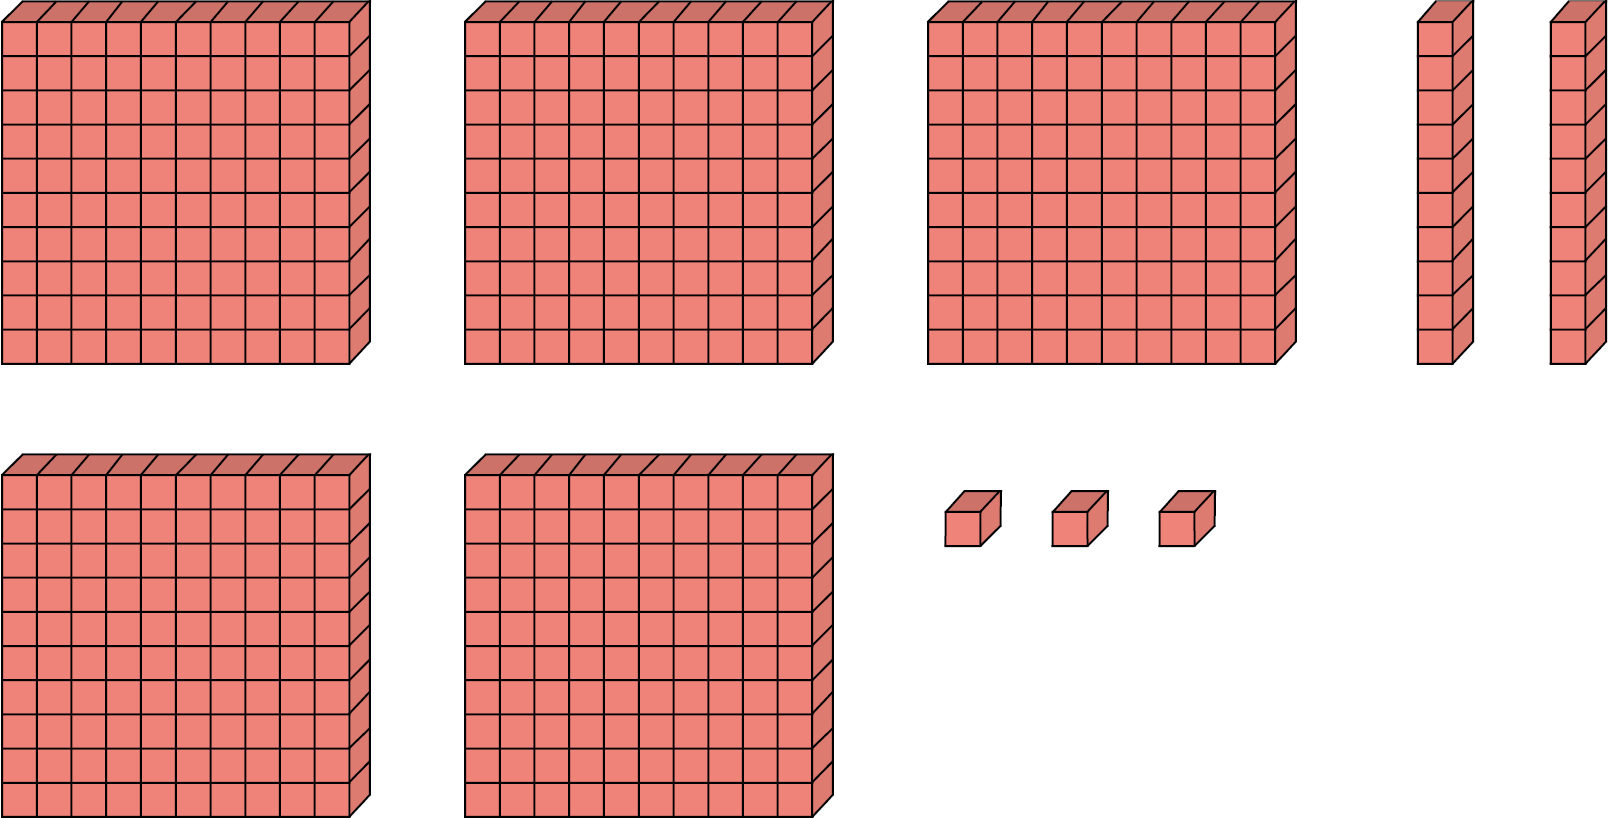
\includegraphics[width=\textwidth]{media/image76.png}
\end{figure}

%Colocar uma placa a mais e 5 barrinhas a mais e 2 unidades a mais

Qual é o número representado pelo material dourado representado na figura?

\begin{escolha}
\item
  523.
\item
  425.
\item
  505.
\item
  525.
\end{escolha}


\num{2} Alex estava jogando dardos em um alvo que possuía áreas de pontuação e,
durante uma rodada, notou que a expressão 3 x 10.000 + 2 x 1.000 + 5 x
100 + 7 x 10, quando resolvida, gerava exatamente o número de pontos que
ele havia feito naquela rodada. A pontuação de Alex naquela rodado foi

%\begin{multicols}{2}
\begin{escolha}
\item
  17 pontos.
\item
  2.570 pontos.
\item
  3.270 pontos.
\item
  32.570 pontos.
\end{escolha}
%\end{multicols}

\pagebreak
\num{3} José resolveu comprar uma placa com o número 587 para sua casa, mas
não percebeu que o número estava
errado, já que o primeiro e o último algarismo estavam em posições
trocadas. O valor relativo do último algarismo na posição que ele 
deveria ocupar no número correto da casa de José é

%\begin{multicols}{2}
\begin{escolha}
\item
  7.
\item
  70.
\item
  700.
\item
  7.000.
\end{escolha}
%\end{multicols}


\num{4} A escola em que Jaqueline estuda está promovendo uma conscientização de
preservação do meio ambiente com o plantio de mudas de árvores
nativas. Sabe-se que já foram plantadas 1.359 mudas e ainda serão
plantadas 1.246. Quantas mudas ao todo serão plantadas durante esse
evento da escola de Jaqueline?

\begin{figure}[htpb!]
\centering
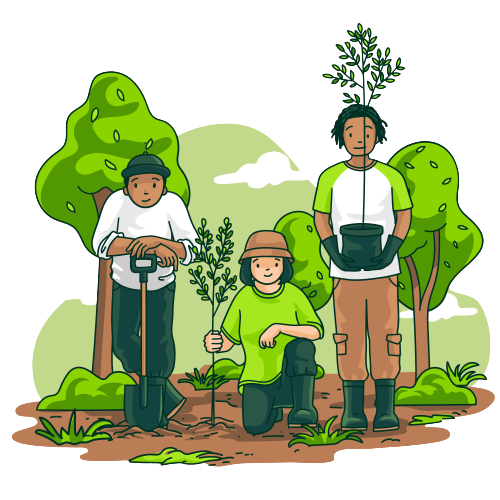
\includegraphics[width=.6\textwidth]{media/image76a.png}
\end{figure}

\begin{multicols}{2}
\begin{escolha}
\item
  113.
\item
  2.523.
\item
  2.605.
\item
  7.052.
\end{escolha}
\end{multicols}

\num{5} Na escola em que André estuda, há 3.452 alunos. Já na escola em que
Pedro estuda, estão matriculados 1.834 alunos. Se, no próximo ano, 300
alunos se matricularem em cada uma das escolas, qual será a diferença
entre a quantidade de alunos das duas escolas?

\begin{multicols}{2}
\begin{escolha}
\item
  2.416.
\item
  1.211.
\item
  1.618.
\item
  1.463.
\end{escolha}
\end{multicols}

\num{6} Ernesto comprou para a festa de aniversário de sua filha 18 litros de
refrigerante e copos descartáveis com capacidade de 250 mililitros.
Quantos copos, com a capacidade máxima tomada por refrigerante, poderão
ser servidos nessa festa considerando-se que Ernesto não comprará mais
refrigerante?

\begin{multicols}{2}
\begin{escolha}
\item
  12.
\item
  36.
\item
  48.
\item
  72.
\end{escolha}
\end{multicols}

\num{7} Observe a figura a seguir, em que cada quadradinho representa uma área de 2 centímetros quadrados.

\begin{figure}[htpb!]
\centering
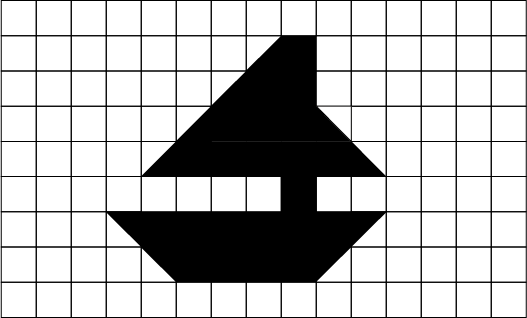
\includegraphics[width=\textwidth]{media/image77.png}
\end{figure}

Considerando-se tudo o que está pintado e juntando-se pedaços
menores para formar quadrados, qual é a área do desenho formado (em centímetros quadrados)?

\begin{escolha}
\item
  24.
\item
  26.
\item
  29.
\item
  58.
\end{escolha}


\num{8} Ana Beatriz e Camila juntaram todo o dinheiro que ganharam de seus pais no
último mês, e as quantias estão representadas a seguir.

\begin{figure}[htpb!]
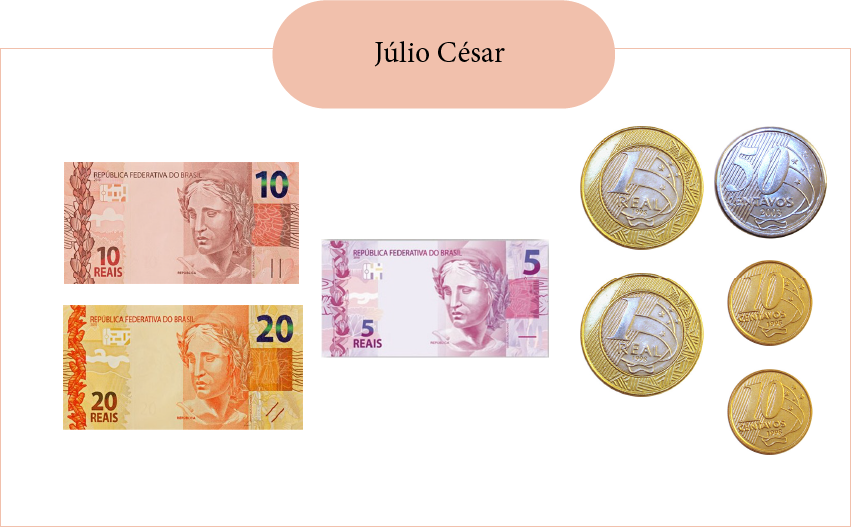
\includegraphics[width=.5\textwidth]{media/image78a.png}
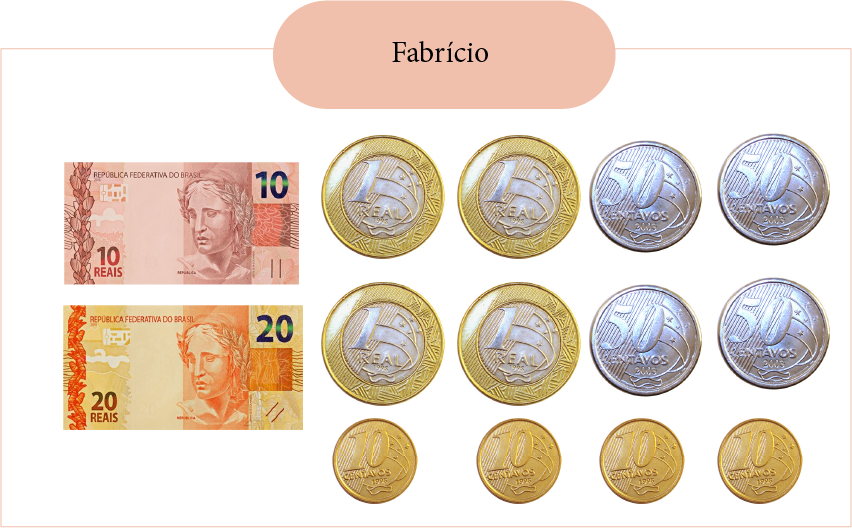
\includegraphics[width=.5\textwidth]{media/image78b.png}
\end{figure}

Qual é o valor total que as duas conseguiram juntar?

\begin{escolha}
\item
  R\$ 93,50.
\item
  R\$ 178,00.
\item
  R\$ 224,00.
\item
  R\$ 300,00.
\end{escolha}


\num{9} A mãe de Isabele está esperando um bebê e hoje será o dia de descobrir
se será menina ou menino. Qual é a probabilidade de Isabele ter um irmão?

\begin{center}
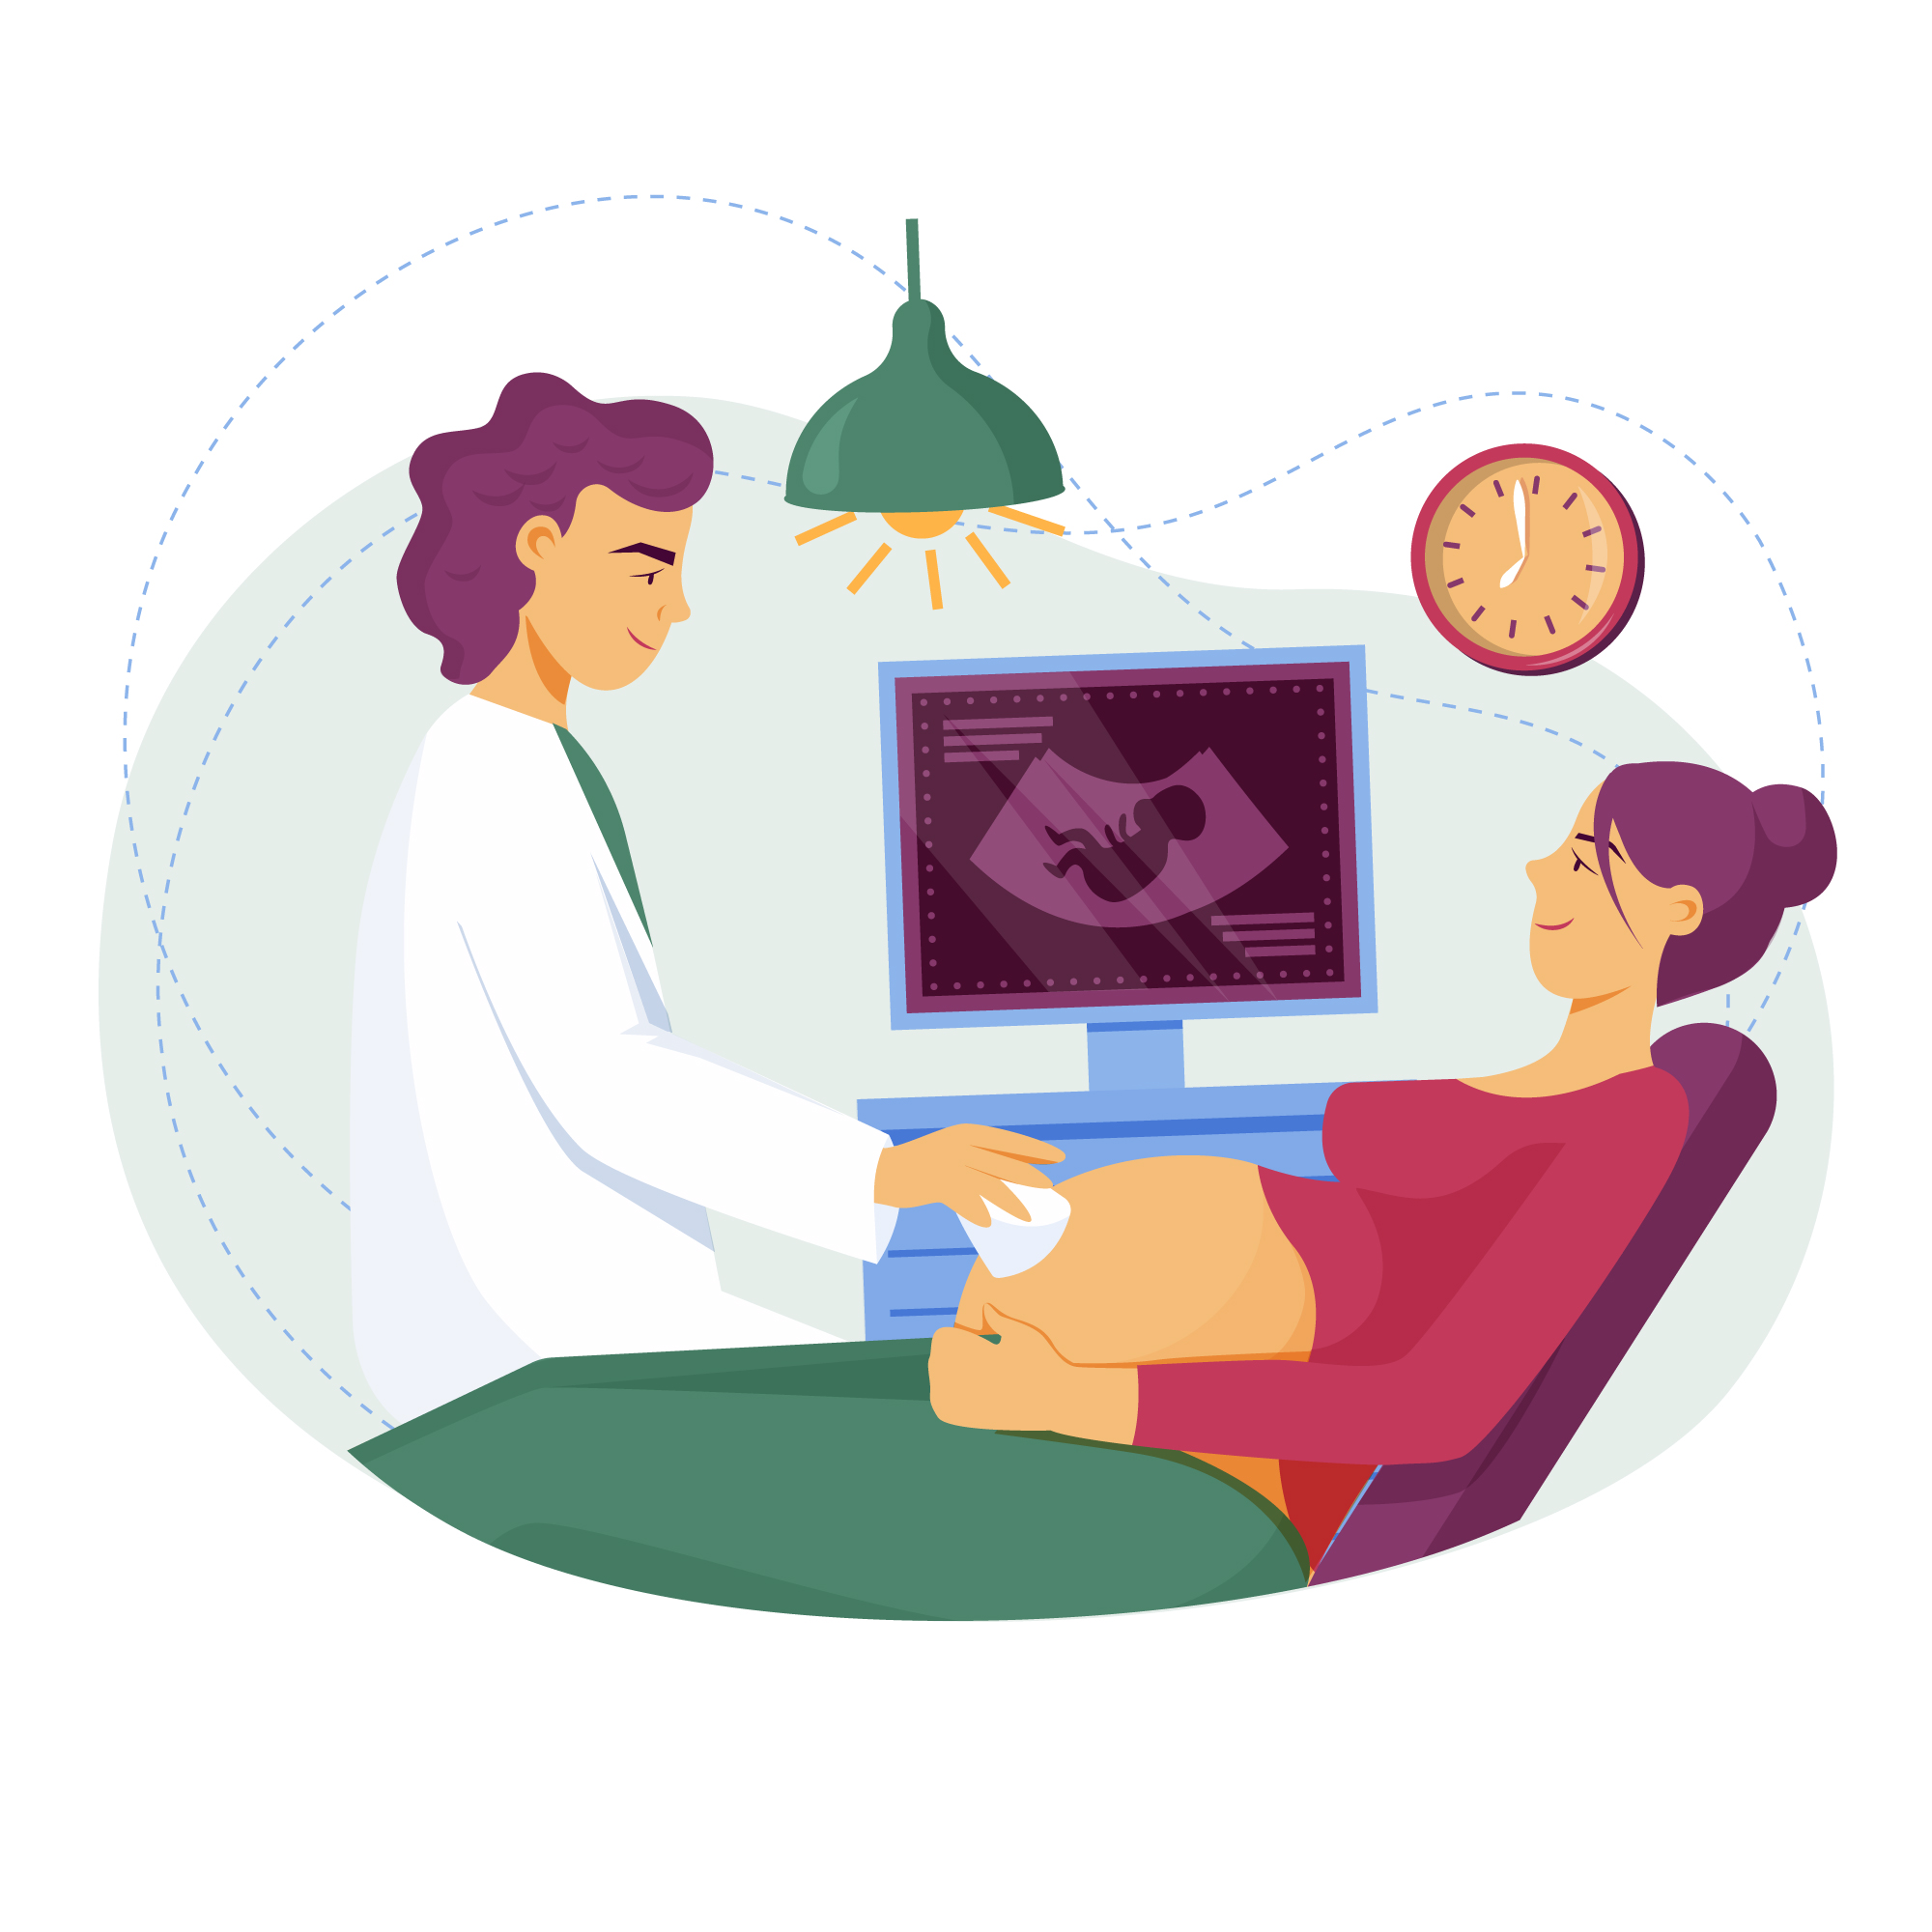
\includegraphics[width=.6\textwidth]{media/image78c.jpeg}
\end{center}

\begin{escolha}
\item
  Nenhuma chance.
\item
  Menos chance do que a de ter uma irmã.
\item
  A mesma chance de ter uma irmã.
\item
  Chance total.
\end{escolha}

\num{10} O gráfico a seguir mostra a taxa de desemprego de uma grande cidade
brasileira.

\begin{figure}[htpb!]
\centering
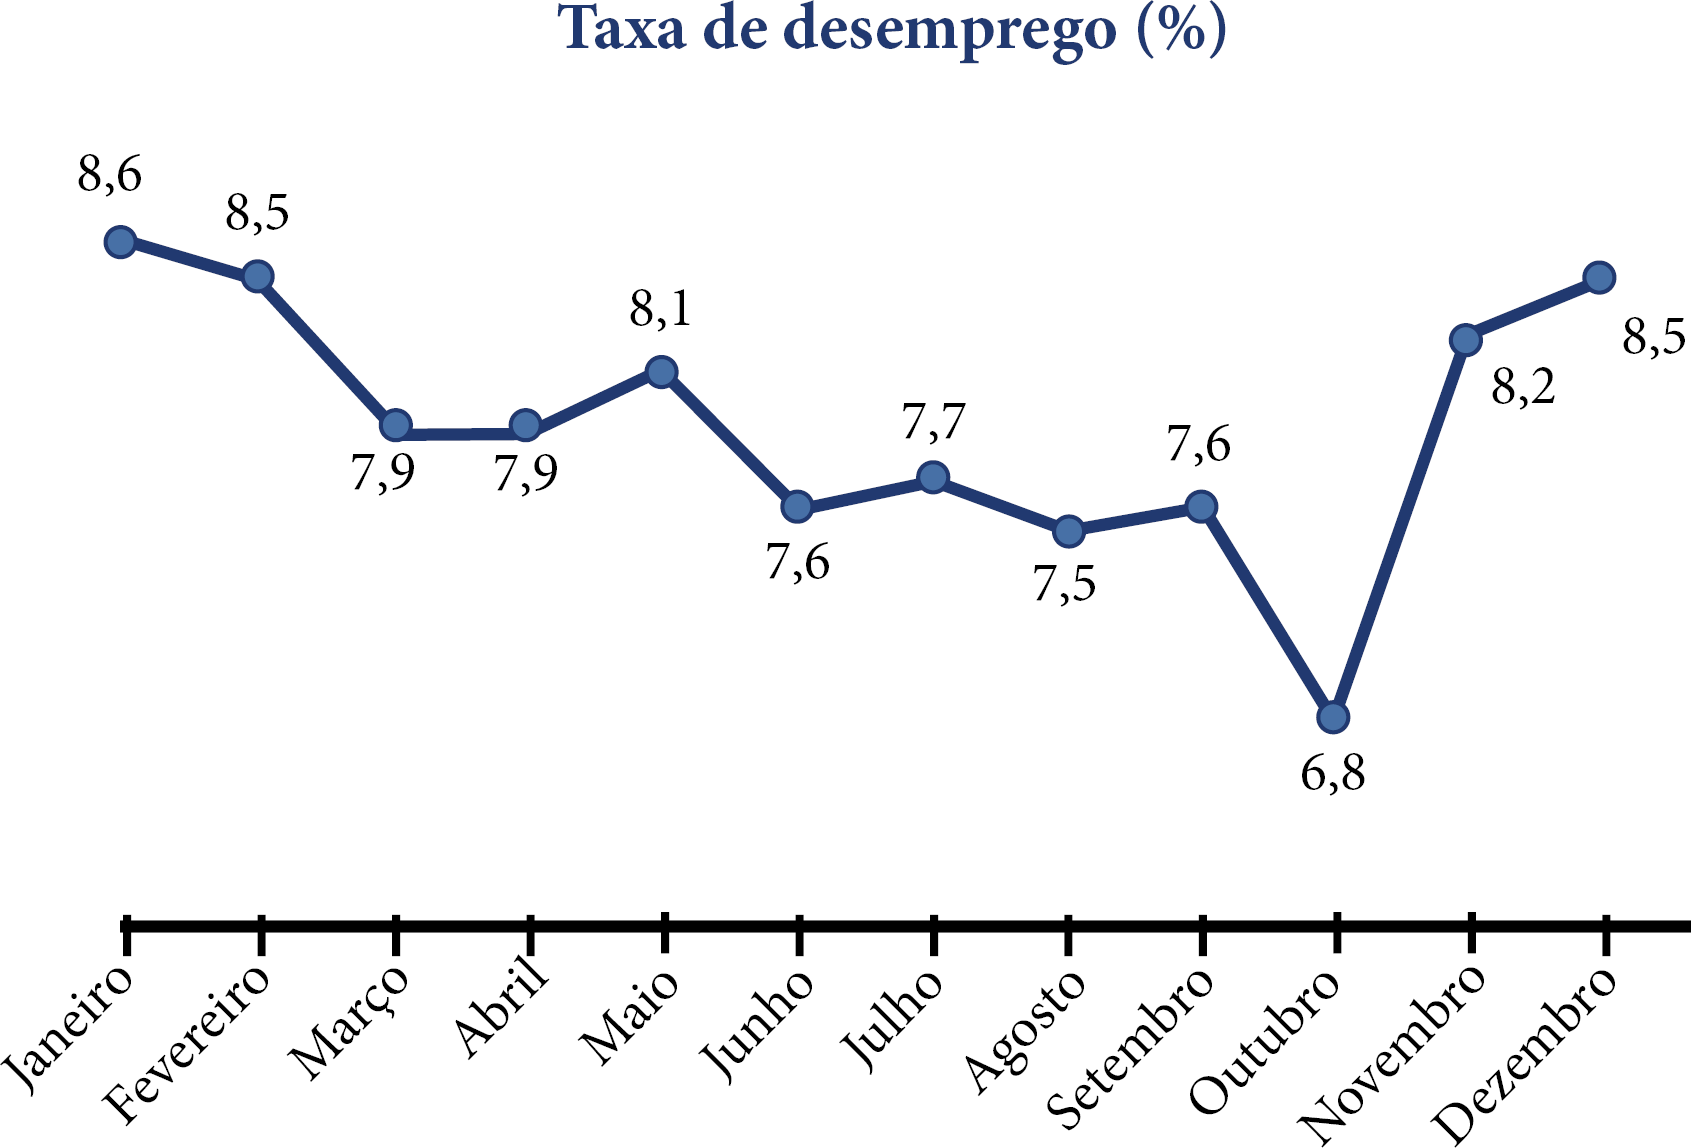
\includegraphics[width=.7\textwidth]{media/image79.png}
\end{figure}

Em que mês houve o maior índice de desemprego?

\begin{multicols}{2}
\begin{escolha}
\item
  Janeiro.
\item
  Julho.
\item
  Outubro.
\item
  Dezembro.
\end{escolha}
\end{multicols}

\num{11} Em um residencial, serão plantadas seis árvores ao lado da rua de comprimento AB. Elas
serão plantadas igualmente espaçadas como se estivessem em uma reta numérica.
Qual é a fração que a distância entre a segunda e a quarta árvore
representa com relação ao tamanho total entre a primeira e a sexta árvore?

%\begin{multicols}{2}
\begin{escolha}
\item
  $\frac{1}{4}$.
\item
  $\frac{2}{5}$.
\item
  $\frac{1}{3}$.
\item
  $\frac{1}{5}$.
\end{escolha}
%\end{multicols}


\num{12} Juca, a uma velocidade de 80 km/h, costuma gastar 1 hora e 30 minutos
para ir da cidade em que mora até a cidade em que sua avó mora. Se ele,
em certo dia, reduziu a velocidade para 50 km/h, o tempo que gastou no mesmo percurso foi de

\begin{escolha}
\item
  1 horas e 24 minutos.
\item
  1 horas e 40 minutos.
\item
  2 horas e 40 minutos.
\item
  2 horas e 24 minutos.
\end{escolha}


\num{13} De quantas maneiras diferentes uma pessoa pode se vestir tendo à
disposição 32 camisetas e 15 bermudas?

\begin{multicols}{2}
\begin{escolha}
\item
  50.
\item
  135.
\item
  385.
\item
  480.
\end{escolha}
\end{multicols}

\num{14} 141,1 litros de suco de laranja dever ser imediatamente colocados,
igualmente, em 17 tambores. Quantos litros de suco de laranja serão
colocados em cada tambor?

\begin{escolha}
\item
  5 litros e 30 mililitros.
\item
  6 litros e 30 mililitros.
\item
  7 litros e 300 mililitros.
\item
  8 litros e 300 mililitros.
\end{escolha}

\num{15} Leia os números apresentados a seguir.

\conteudo{
\textit{}

\textbf{15.610}

\textbf{3.456}

\textbf{1.278}

\textbf{10.321}
}

Colocados nessa ordem, como um desses números está corretamente escrito?

\begin{escolha}
\item Mil, quinhentos e dez.

\item Três mil, quatrocentos e cinquenta e seis.

\item Doze mil, setecentos e oito.

\item Dez mil, trezentos e doze.
\end{escolha}
\pagebreak

\vspace*{-3.4cm}
\hspace*{-3.7cm}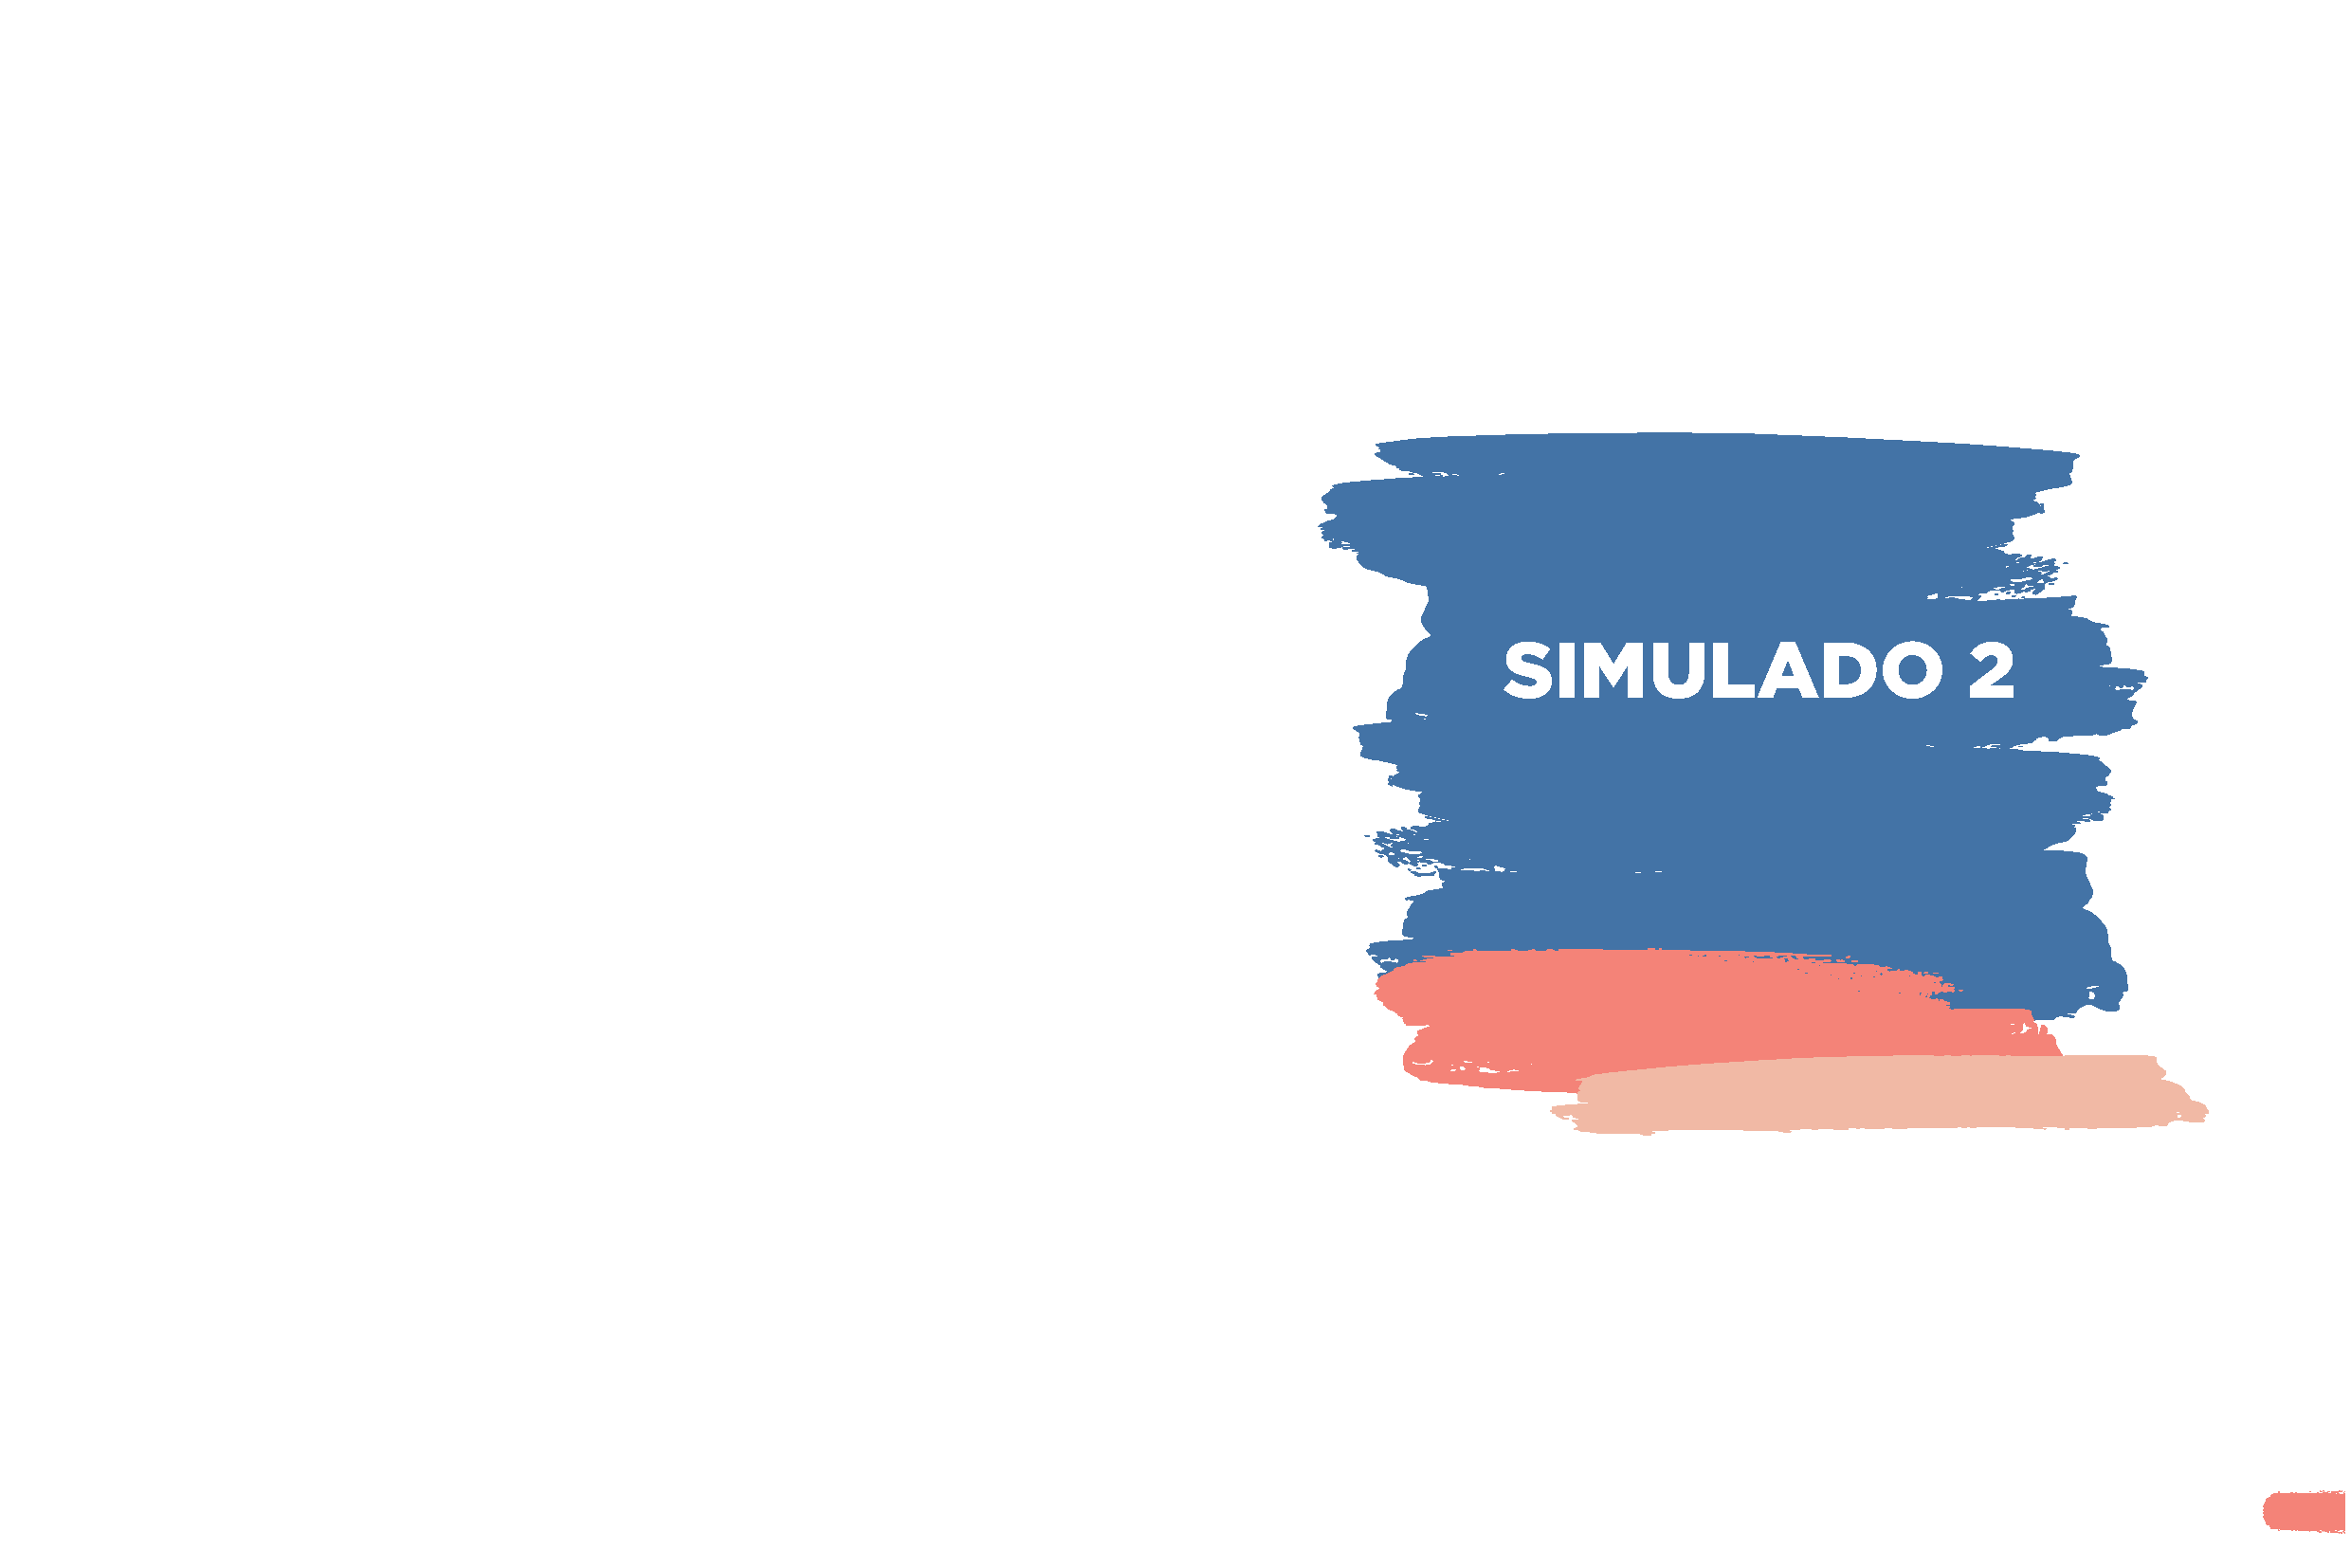
\includegraphics[scale=1]{../watermarks/2simulado5ano.pdf}
\addcontentsline{toc}{chapter}{Simulado 2}
\markboth{Simulado 2}{}
\pagebreak

\num{1} Utilizando um ábaco, Miguel representou o seguinte número:

\begin{figure}[htpb!]
\centering

\includegraphics[width=\textwidth]{media/image80.png}
\end{figure}

Qual foi o número que Miguel representou?

\begin{multicols}{2}
\begin{escolha}
\item
  1.314.
\item
  4.131.
\item
  20.314.
\item
  10.314.
\end{escolha}
\end{multicols}

\num{2} Isabele quer colocar o número 364 em uma reta numérica segmentada de 50 em 50 unidades partindo do 100 e chegando ao 500. O número 364 deve aparecer

\begin{multicols}{2}
\begin{escolha}
\item
  150 e 200.
\item
  250 e 300.
\item
  350 e 400.
\item
  450 e 500.
\end{escolha}
\end{multicols}

\num{3} Analise a sequência a seguir.

\conteudo{
\textbf{340; 280; 220; 160; ...}
}

O próximo número será o

\begin{multicols}{2}
\begin{escolha}
\item
  100.
\item
  60.
\item
  40.
\item
  20.
\end{escolha}
\end{multicols}

\pagebreak
\num{4} Veja o que disse Raquel.

\conteudo{
\textbf{Vou completar 13 anos daqui a 7 semanas e 3 dias.}
}

Quantos dias faltam no total?

\begin{multicols}{2}
\begin{escolha}
\item
  52.
\item
  43.
\item
  32.
\item
  17.
\end{escolha}
\end{multicols}

\num{5} Um lote de 26.104 lápis será embalado em caixas contendo 52 unidades cada. Essas caixas serão distribuídas uma para cada escola
estadual que existe na região em que Lucas mora. Quantas escolas
receberão uma caixa contendo lápis?

\begin{figure}[htpb!]
\centering
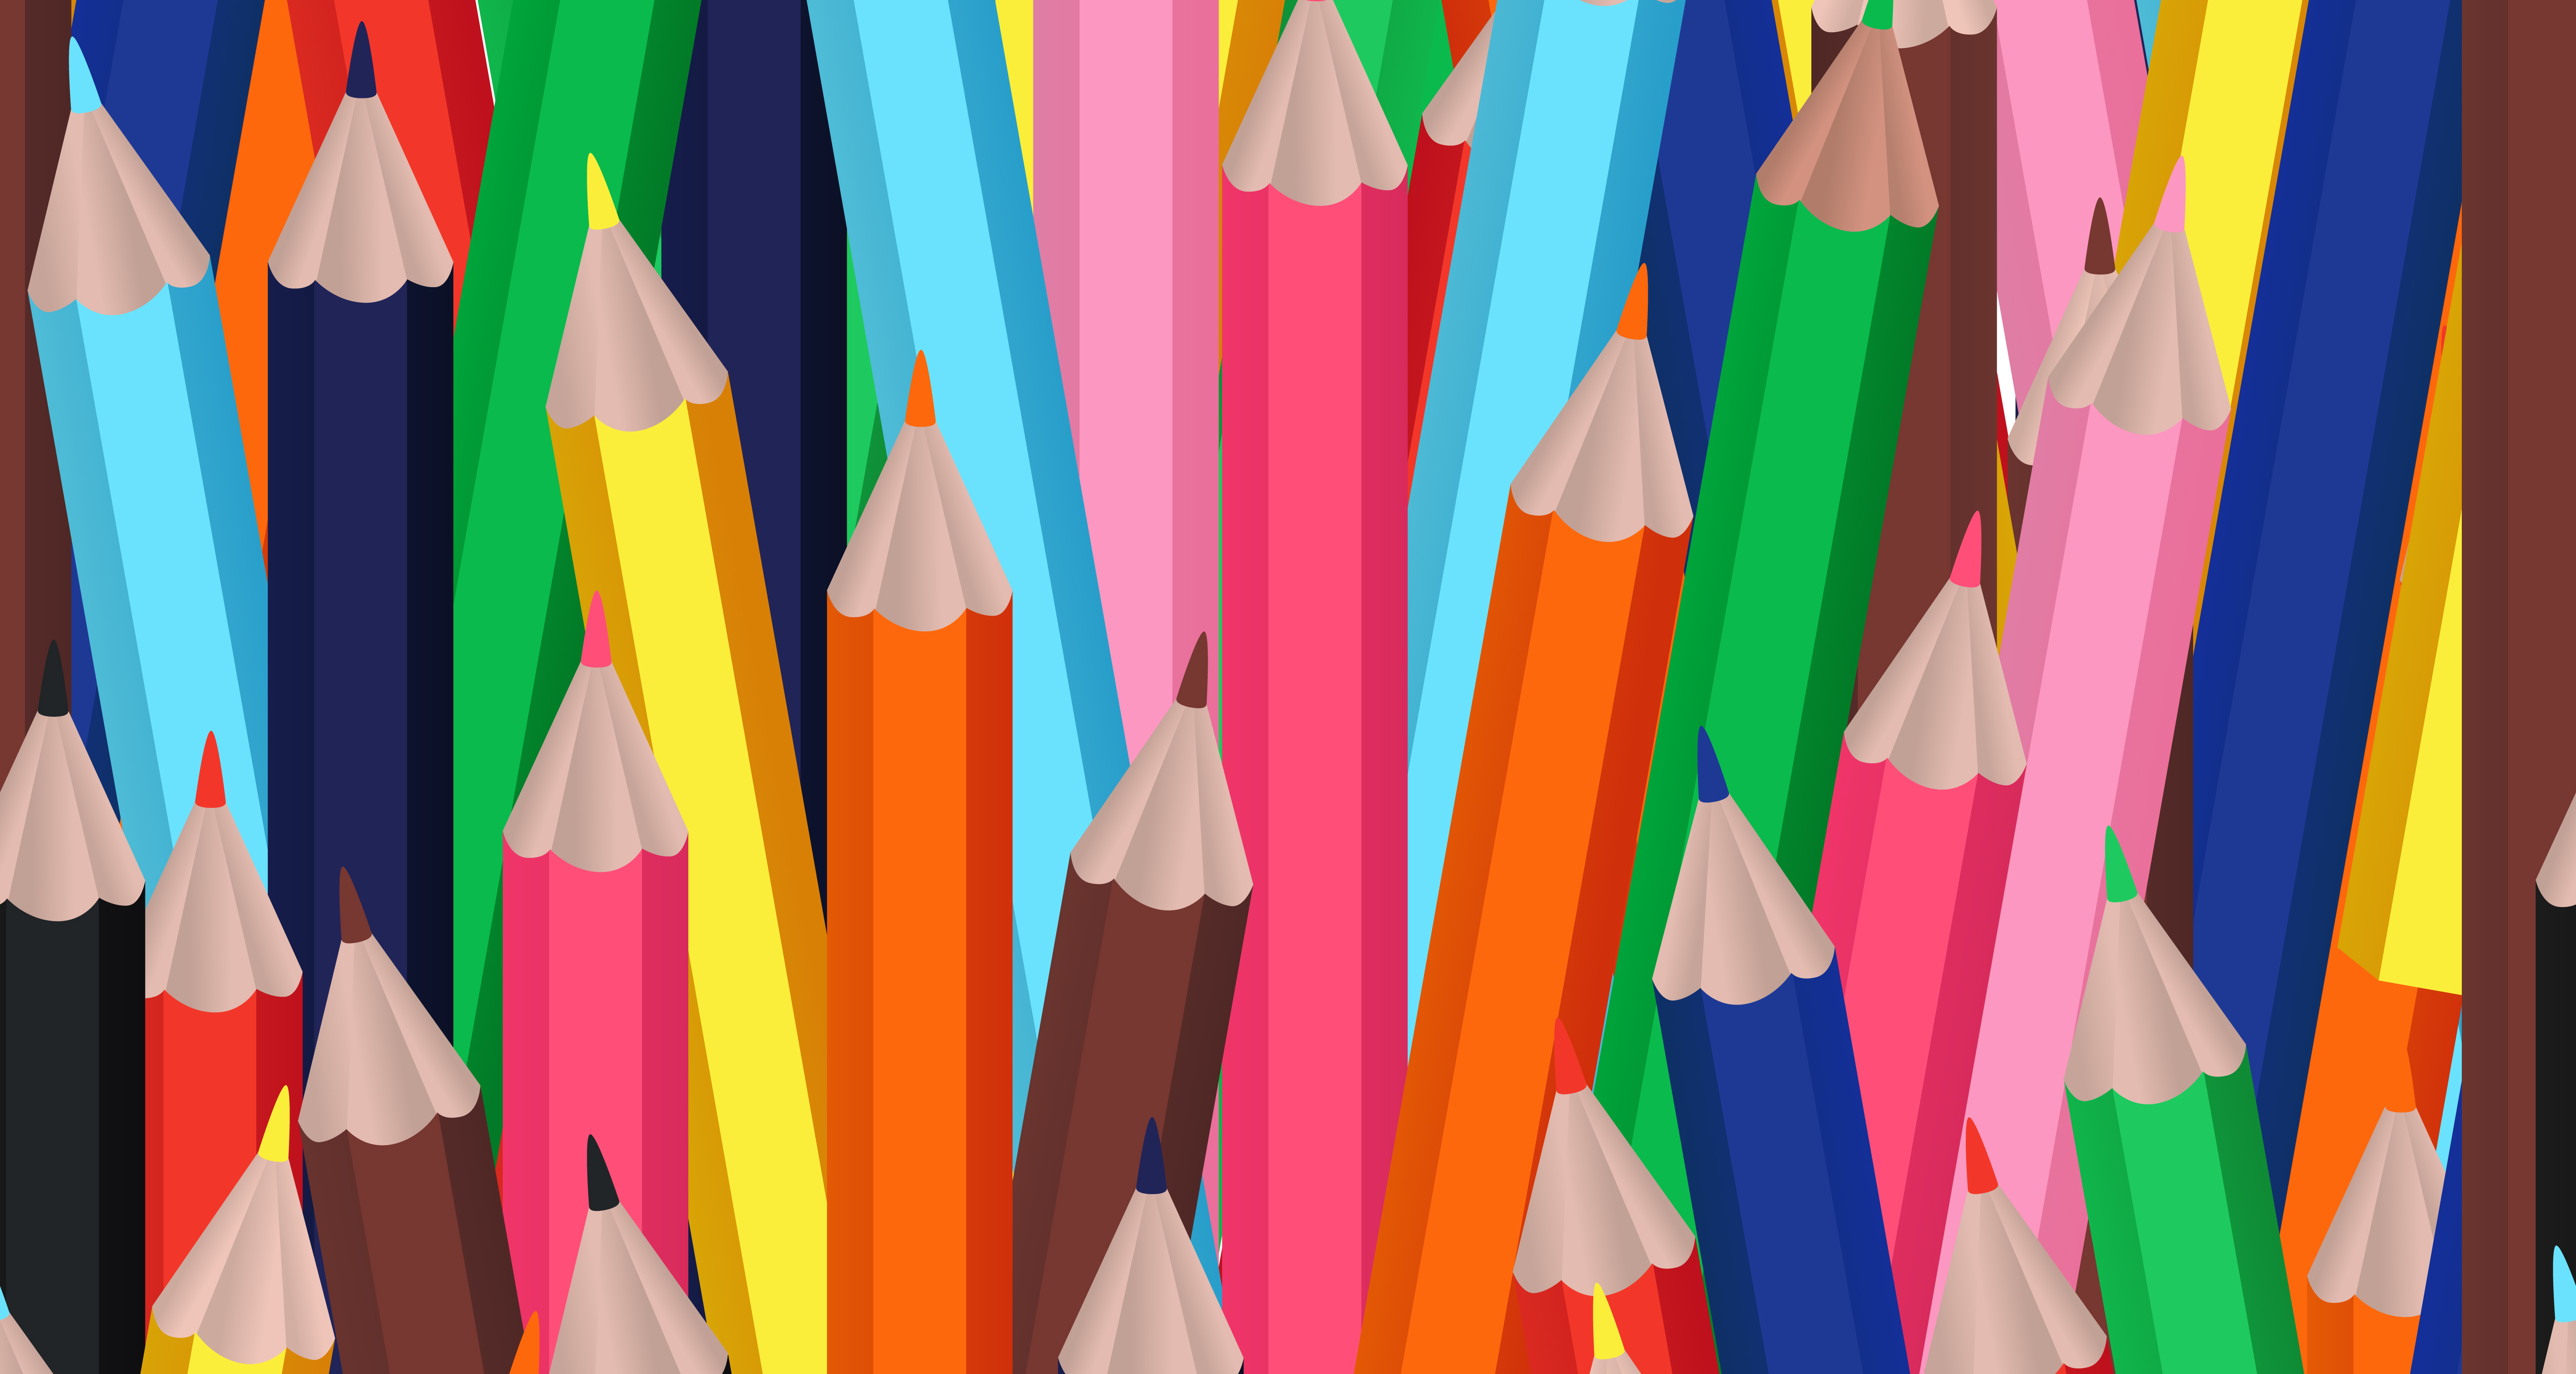
\includegraphics[width=.9\textwidth]{media/image80a.jpeg}
\end{figure}

\begin{multicols}{2}
\begin{escolha}
\item
  126.
\item
  208.
\item
  502.
\item
  2.008.
\end{escolha}
\end{multicols}

\num{6} Um marceneiro quer medir uma tábua, mas esqueceu sua trena. Dessa
forma, resolveu medir com seu palmo, que mede aproximadamente 21 cm, e
chegou à conclusão de que a tábua possui o comprimento
de 7 palmos seus. A tábua tem uma medida aproximada de

\begin{multicols}{2}
\begin{escolha}
\item
  1,10 m.
\item
  1,40 m.
\item
  1,50 m.
\item
  1,60 m.
\end{escolha}
\end{multicols}

\num{7} Com uma fita, Jonas está marcando no chão a letra inicial do nome de sua mãe. Veja a seguir.

\begin{figure}[htpb!]
\centering
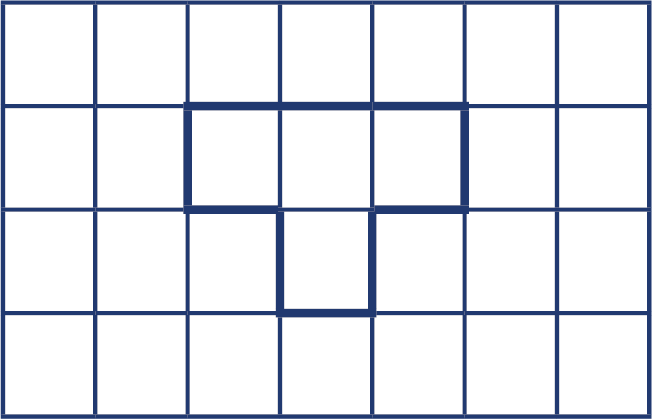
\includegraphics[width=\textwidth]{media/image81.png}
\end{figure}

Cada lado do quadrado que forma o piso mede 1,2 m de
comprimento. De quantos metros de fita Jonas precisará para concluir seu
trabalho, se dará três voltas com a fita em torno da letra?

\begin{multicols}{2}
\begin{escolha}
\item
  36.
\item
  18.
\item
  12.
\item
  6.
\end{escolha}
\end{multicols}


\num{8} Vanessa foi a uma loja de material escolar e comprou uma mochila por R\$ 103,00 e uma lancheira por R\$ 59,00. Qual foi o valor da compra realizada por Vanessa?

\begin{multicols}{2}
\begin{escolha}
\item
  R\$ 113,00
\item
  R\$ 133,80
\item
  R\$ 162,00
\item
  R\$ 173,80
\end{escolha}
\end{multicols}


\num{9} Amanda acaba de jogar um dado de seis faces, em que cada face
há um número natural distinto de 1 a 6. Qual é a probabilidade de, na
face voltada para cima, sair um número menor que 0 ou igual a 0?

\begin{multicols}{2}
\begin{escolha}
\item
  Nada provável.
\item
  Pouco provável.
\item
  Muito provável.
\item
  Totalmente certo.
\end{escolha}
\end{multicols}

\num{10} Três alunos realizaram 5 provas cada um e as notas obtidas por eles se
encontram na tabela a seguir.

\begin{figure}[htpb!]
\centering
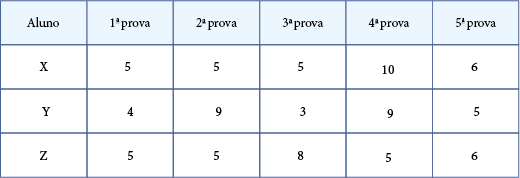
\includegraphics[width=\textwidth]{media/image82.png}
\end{figure}

O aluno que será classificado será aquele que tiver a maior
soma de todas as notas. O terceiro lugar será do aluno

\begin{multicols}{2}
\begin{escolha}
\item
  X.
\item
  Y.
\item
  Z.
\item
  X ou Z.
\end{escolha}
\end{multicols}

\num{11} Gabriel ganhou de sua avó uma barra de chocolate com quatro quadradinhos na largura e cinco quadradinos no comprimento.
O número de quadradinhos que ele deverá comer para consumir $\frac{2}{5}$ do total
da barra de chocolate é

\begin{multicols}{2}
\begin{escolha}
\item
  3.
\item
  8.
\item
  12.
\item
  15.
\end{escolha}
\end{multicols}

\num{12} Maria é especialista em fazer um café delicioso. Na receita dela, é utilizada uma colher de sopa de pó de café para cada 250 mL
de água. Quantas colheres de sopa de pó de café deverão ser utilizadas, seguindo a receita de Maria, se a quantidade de água for de 1.250 mL de água?

\begin{multicols}{2}
\begin{escolha}
\item
  2.
\item
  3.
\item
  4.
\item
  5.
\end{escolha}
\end{multicols}


\num{13} Para uma competição de xadrez, foram inscritos 22 jogadores. Quantas são
as possibilidades de se formar o pódio com o resultado final, ou seja,
primeiro, segundo e terceiro lugares?

\begin{multicols}{2}
\begin{escolha}
\item
  1.690.
\item
  3.600.
\item
  9.240.
\item
  10.000.
\end{escolha}
\end{multicols}

\num{14} Pela manhã, Ricardo abasteceu o carro, pois o tanque estava totalmente
vazio. Ele gastou R\$ 208,00 para encher o tanque completamente.
O preço do litro do combustível utilizado por Ricardo
é de R\$ 4,00. Quantos litros de combustível couberam no tanque do carro de
Ricardo?

\begin{multicols}{2}
\begin{escolha}
\item
  25.
\item
  34.
\item
  46.
\item
  52.
\end{escolha}
\end{multicols}

\num{15} Leia, a seguir, alguns números escritos por extenso.

\begin{itemize}
\item Sete mil e quinhentos.

\item Vinte e um mil, duzentos e setenta e sete.

\item Treze mil, quatrocentos e oito.

\item Mil, seiscentos e oitenta e quatro.
\end{itemize}\enlargethispage{\baselineskip}

Colocados nessa ordem, um número em algarismos que está escrito nessa lista é

\begin{multicols}{2}
\begin{escolha}
\item 7.005.
\item 21.277.
\item 13.480.
\item 16.840.
\end{escolha}
\end{multicols}
\pagebreak

\vspace*{-3.4cm}
\hspace*{-3.7cm}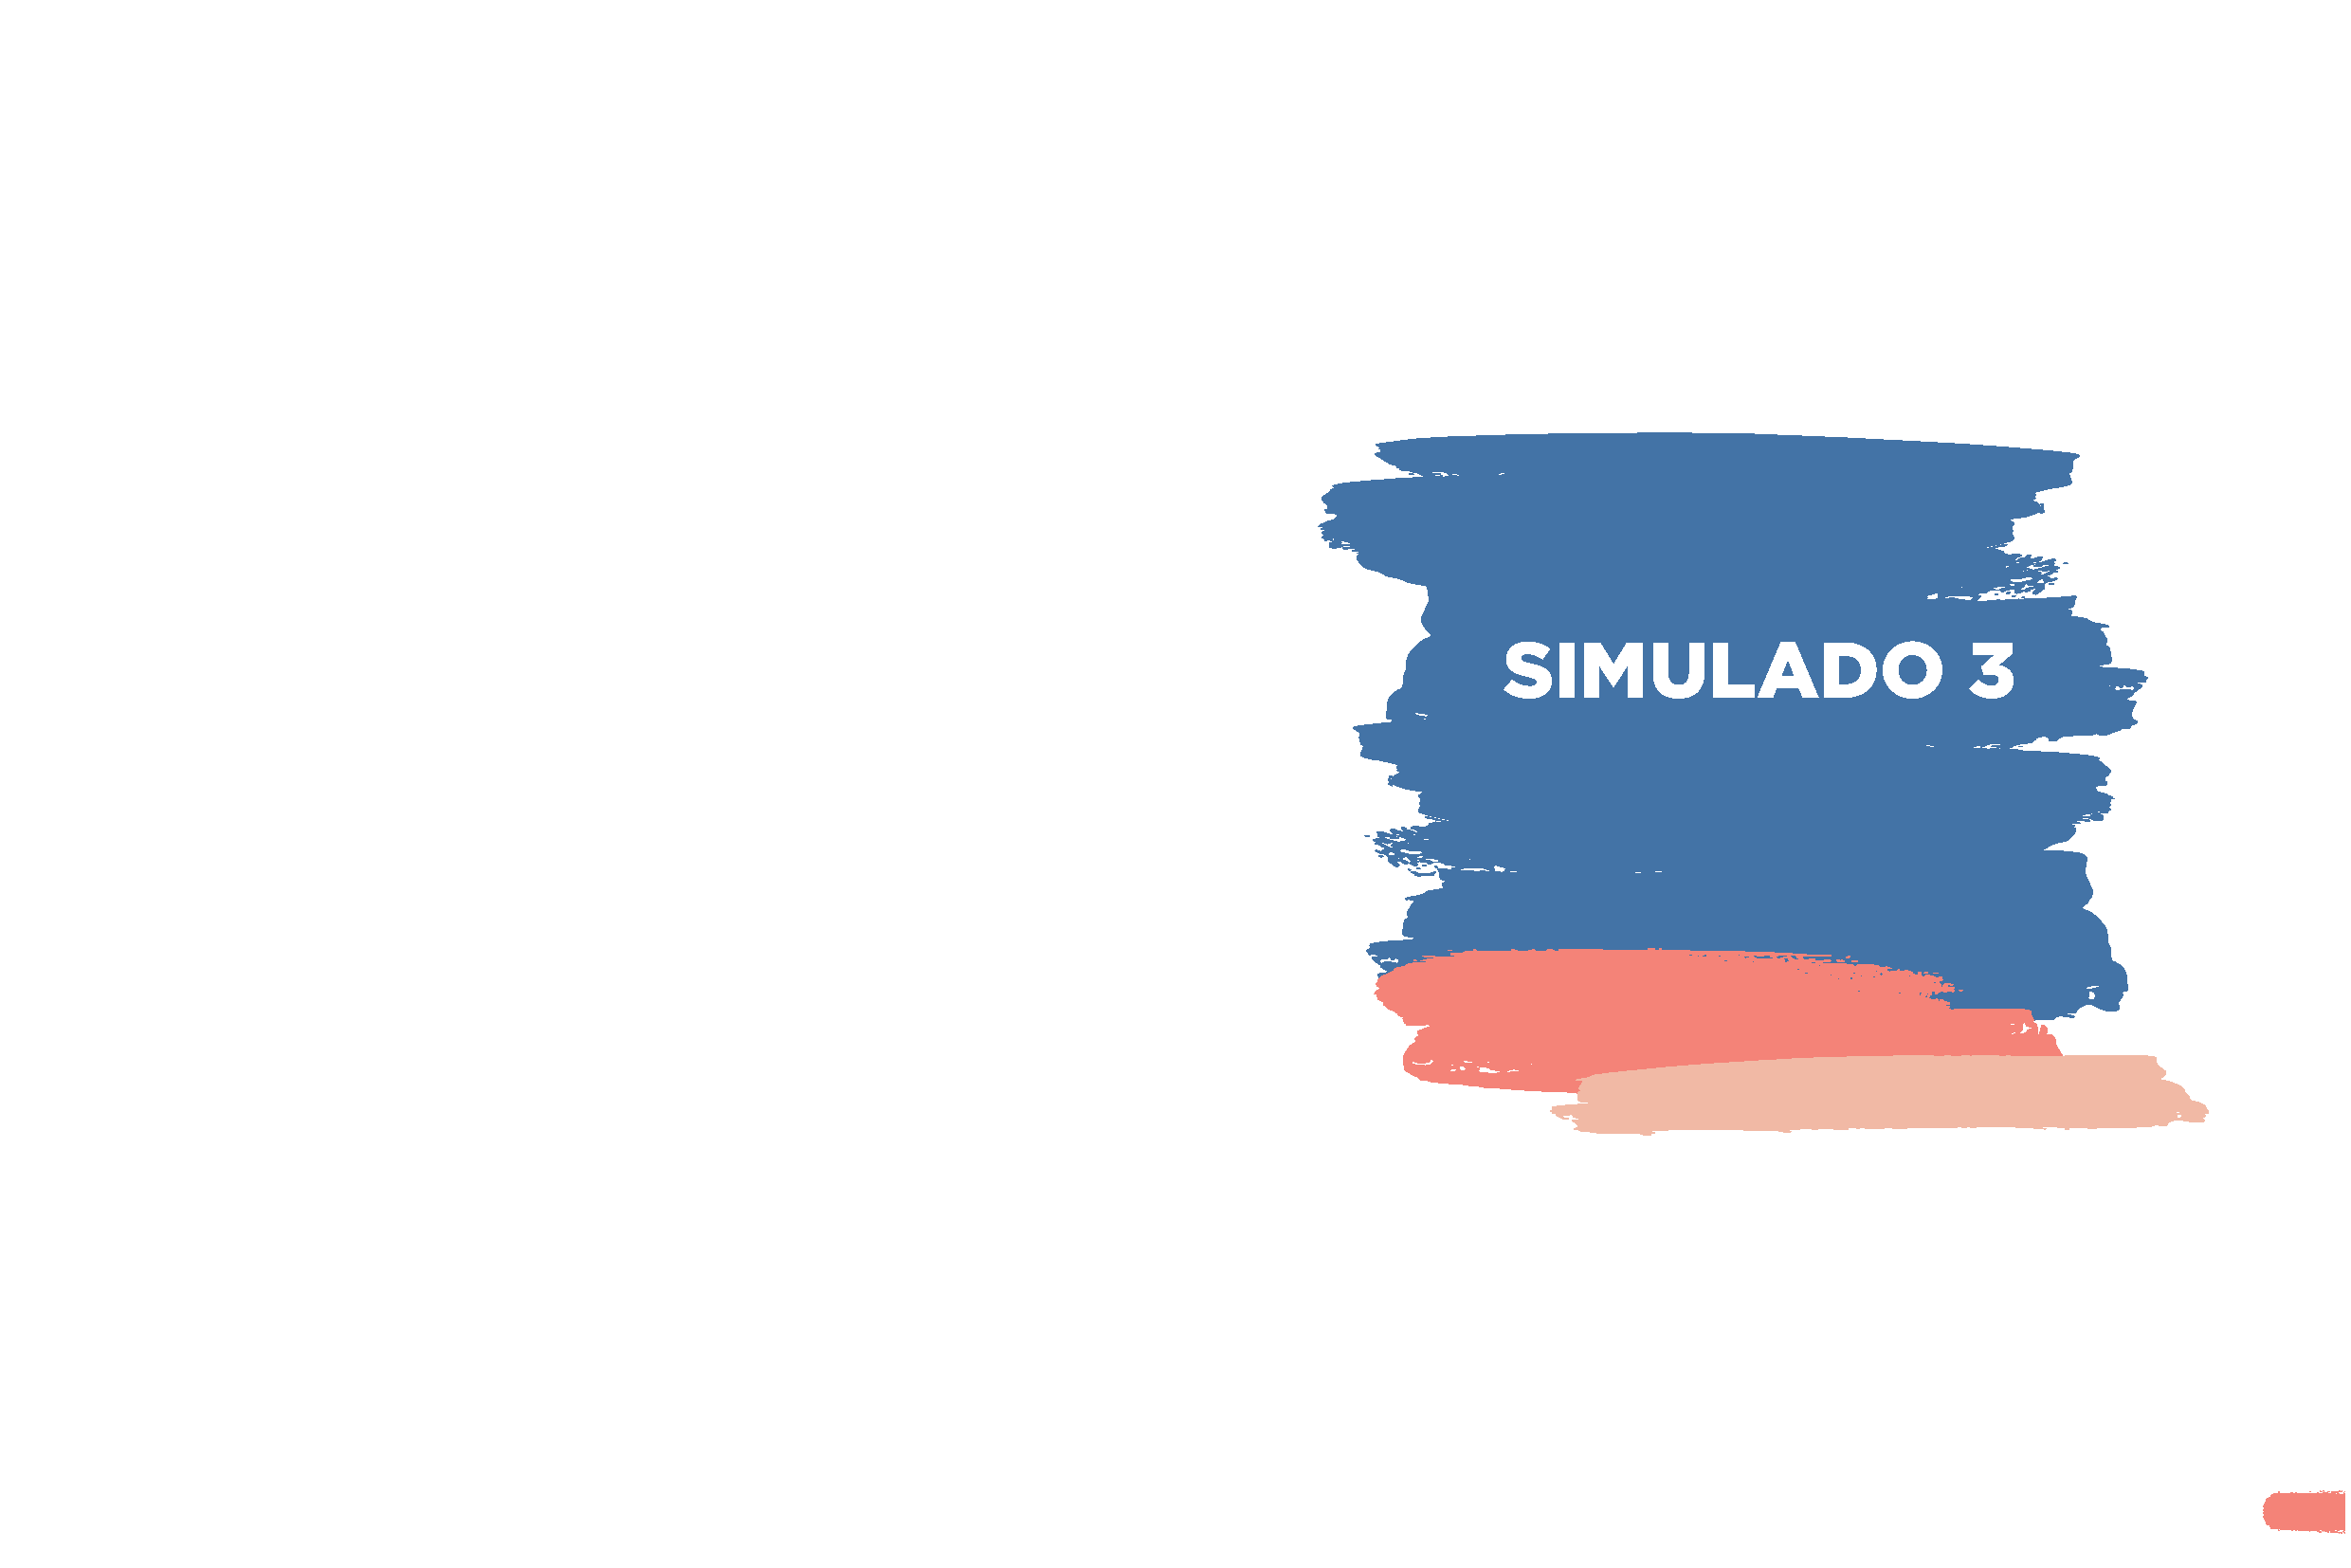
\includegraphics[scale=1]{../watermarks/3simulado5ano.pdf}
\addcontentsline{toc}{chapter}{Simulado 3}
\markboth{Simulado 3}{}
\pagebreak

\num{1} Durante a aula de Matemática, a professora colocou na lousa a seguinte
decomposição de um número.

\conteudo{
\textbf{5 x 10.000 + 3 x 1.000 + 3 x 100 + 5 x 10}
}

Muito rapidamente, Artur levantou a mão e disse que sabia qual era o
número. Qual é o número representado por essa decomposição?

\begin{escolha}
\item
  35.250.
\item
  3.535.
\item
  5.035.
\item
  53.350.
\end{escolha}


\num{2} Ricardo deseja escrever o segundo maior número que se pode escrever
utilizando os algarismos 1, 2, 4, 5 e 7 sem repeti-los nenhuma vez.
Que número é esse?

\begin{escolha}
\item
  Setecentos e cinquenta mil e quatrocentos e vinte um.
\item
  Setenta e cinco mil e quatrocentos e doze.
\item
  Quarenta e cinco mil e duzentos e cinquenta e sete.
\item
  Dezessete mil e quinhetos e quarenta e cinco.
\end{escolha}


\num{3} A seguinte conta foi colocada no quadro durante uma aula de Matemática.

\begin{figure}[htpb!]
\centering
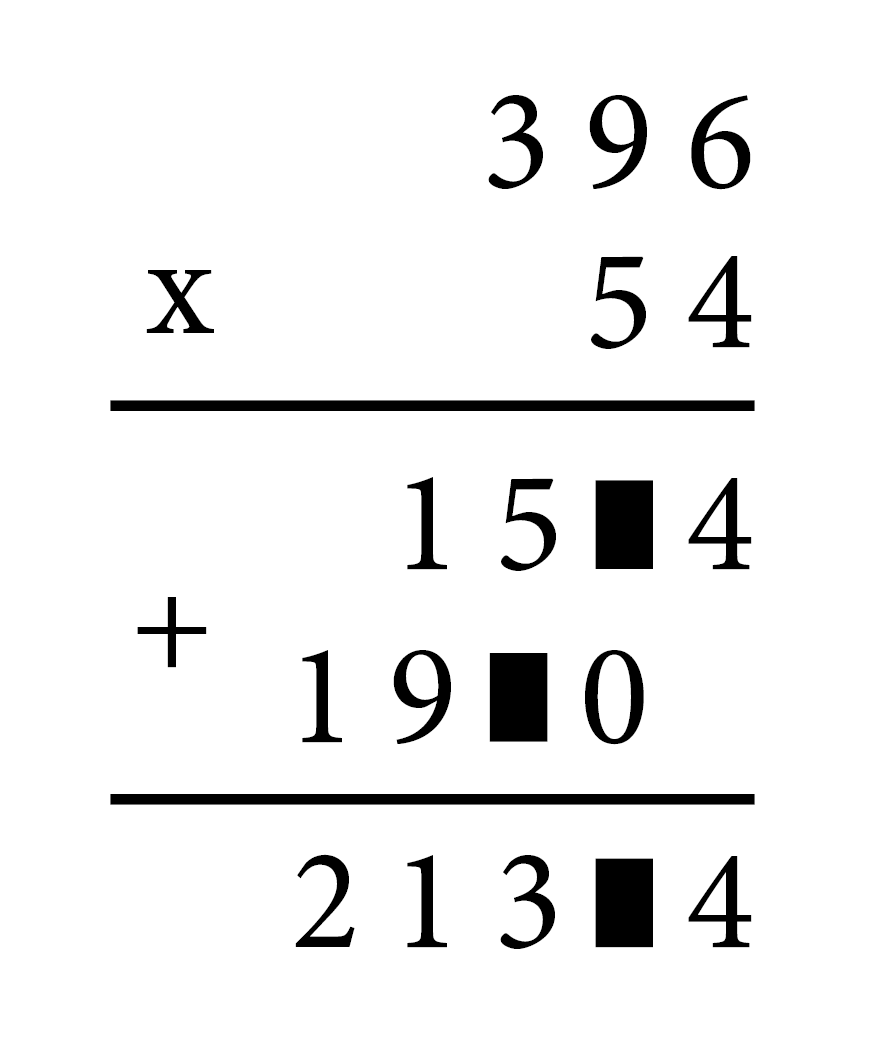
\includegraphics[width=.25\textwidth]{media/image83.png}
\end{figure}

\pagebreak
Que número devemos colocar no lugar dos quadradinhos para que a conta
fique correta?

\begin{multicols}{2}
\begin{escolha}
\item
  2.
\item
  6.
\item
  7.
\item
  8.
\end{escolha}
\end{multicols}

\num{4} Alex estava observando a sequência numérica (3; 9; 27, 81; 243; 729).
Ele percebeu que, para encontrar um elemento qualquer da sequência,
deveria

\begin{escolha}
\item
  somar 6 a um termo anterior.
\item
  dividir um termo anterior por 3.
\item
  multiplicar um termo anterior por 3.
\item
  somar 9 a um termo anterior.
\end{escolha}


\num{5} O zoológico da cidade em que Fabiana mora abre às 9h25 da manhã e fica
aberto apenas 7 horas e meia por dia Qual é o horário em que o zoológico
fecha, sabendo-se que ele não fecha no horário do almoço?

\vspace{2em}
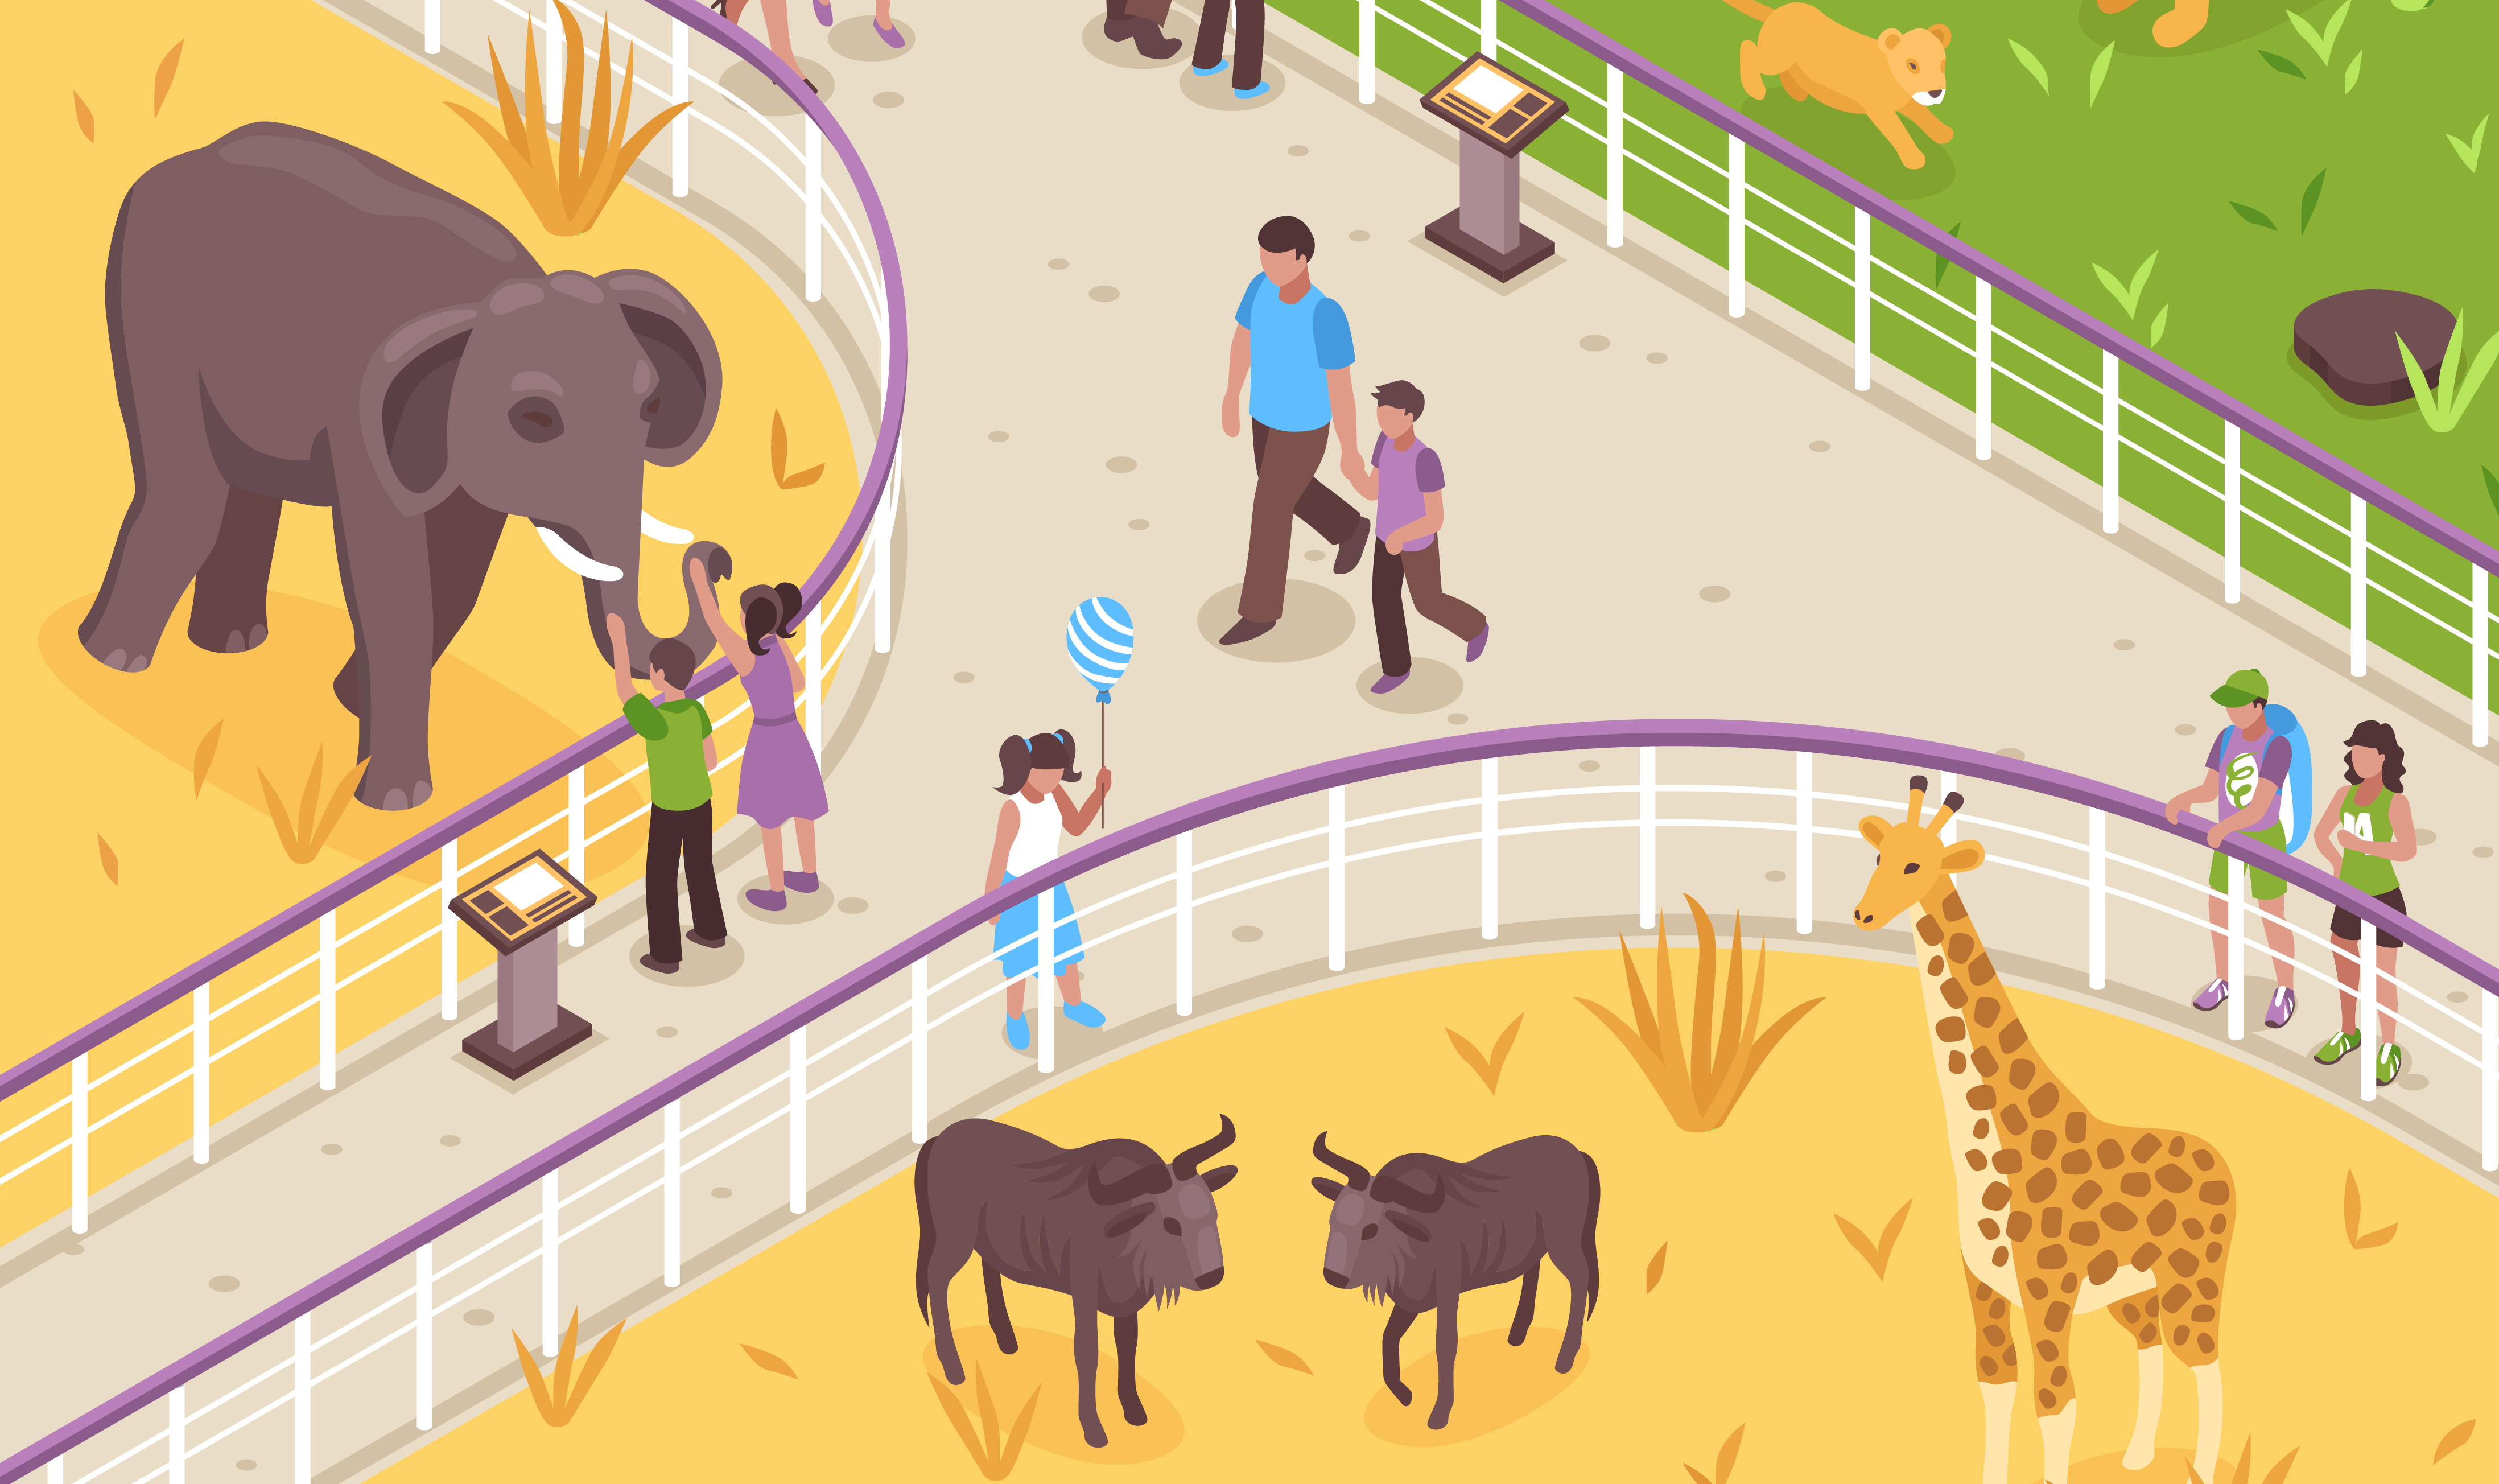
\includegraphics[width=\textwidth]{media/image83a.jpeg}

\begin{multicols}{2}
\begin{escolha}
\item
  16h30.
\item
  17h30.
\item
  16h45.
\item
  18h30.
\end{escolha}
\end{multicols}

\num{6} O programa preferido de Marquinhos na TV começa pontualmente às 13
horas e 55 minutos e termina exatamente às 15 horas e 39 minutos. Qual é a
duração do programa?


\includegraphics[width=.6\textwidth]{media/image83b.png}

\begin{multicols}{2}
\begin{escolha}
\item
  39 minutos.
\item
  45 minutos.
\item
  50 minutos.
\item
  1 hora e 44 minutos.
\end{escolha}
\end{multicols}

\num{7} Marina quer colocar um carpete de madeira no quarto de sua única filha.
Para isso, representou o quarto da menina na malha quadriculada a seguir, em que a parte escura corresponde ao carpete de madeira que será
colocado.

\begin{figure}[htpb!]
\centering
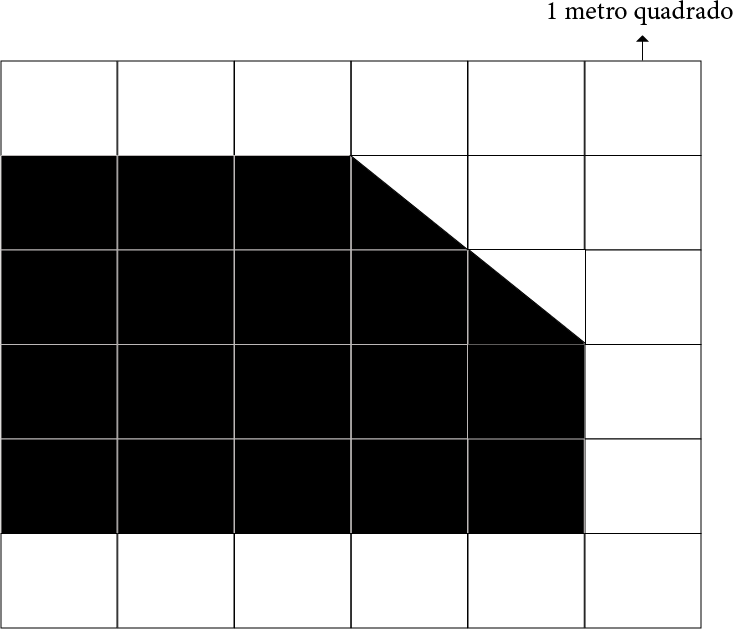
\includegraphics[width=.5\textwidth]{media/image84.png}
\end{figure}

Como cada quadradinho possui 1 metro quadrado de área, qual é a área total
de carpete de madeira que ela terá de encomendar para colocar no quarto
da filha sem que falte nenhum pedaço e também não sobre material?

\begin{multicols}{2}
\begin{escolha}
\item
  12 metros quadrados.
\item
  17 metros quadrados.
\item
  18 metros quadrados.
\item
  20 metros quadrados.
\end{escolha}
\end{multicols}

\num{8} Um cartão é retirado de forma aleatória de um conjunto de 50 cartões
numerados de 1 a 50. Qual é a probabilidade de que no cartão retirado
tenha escrito um número par?

\begin{center}
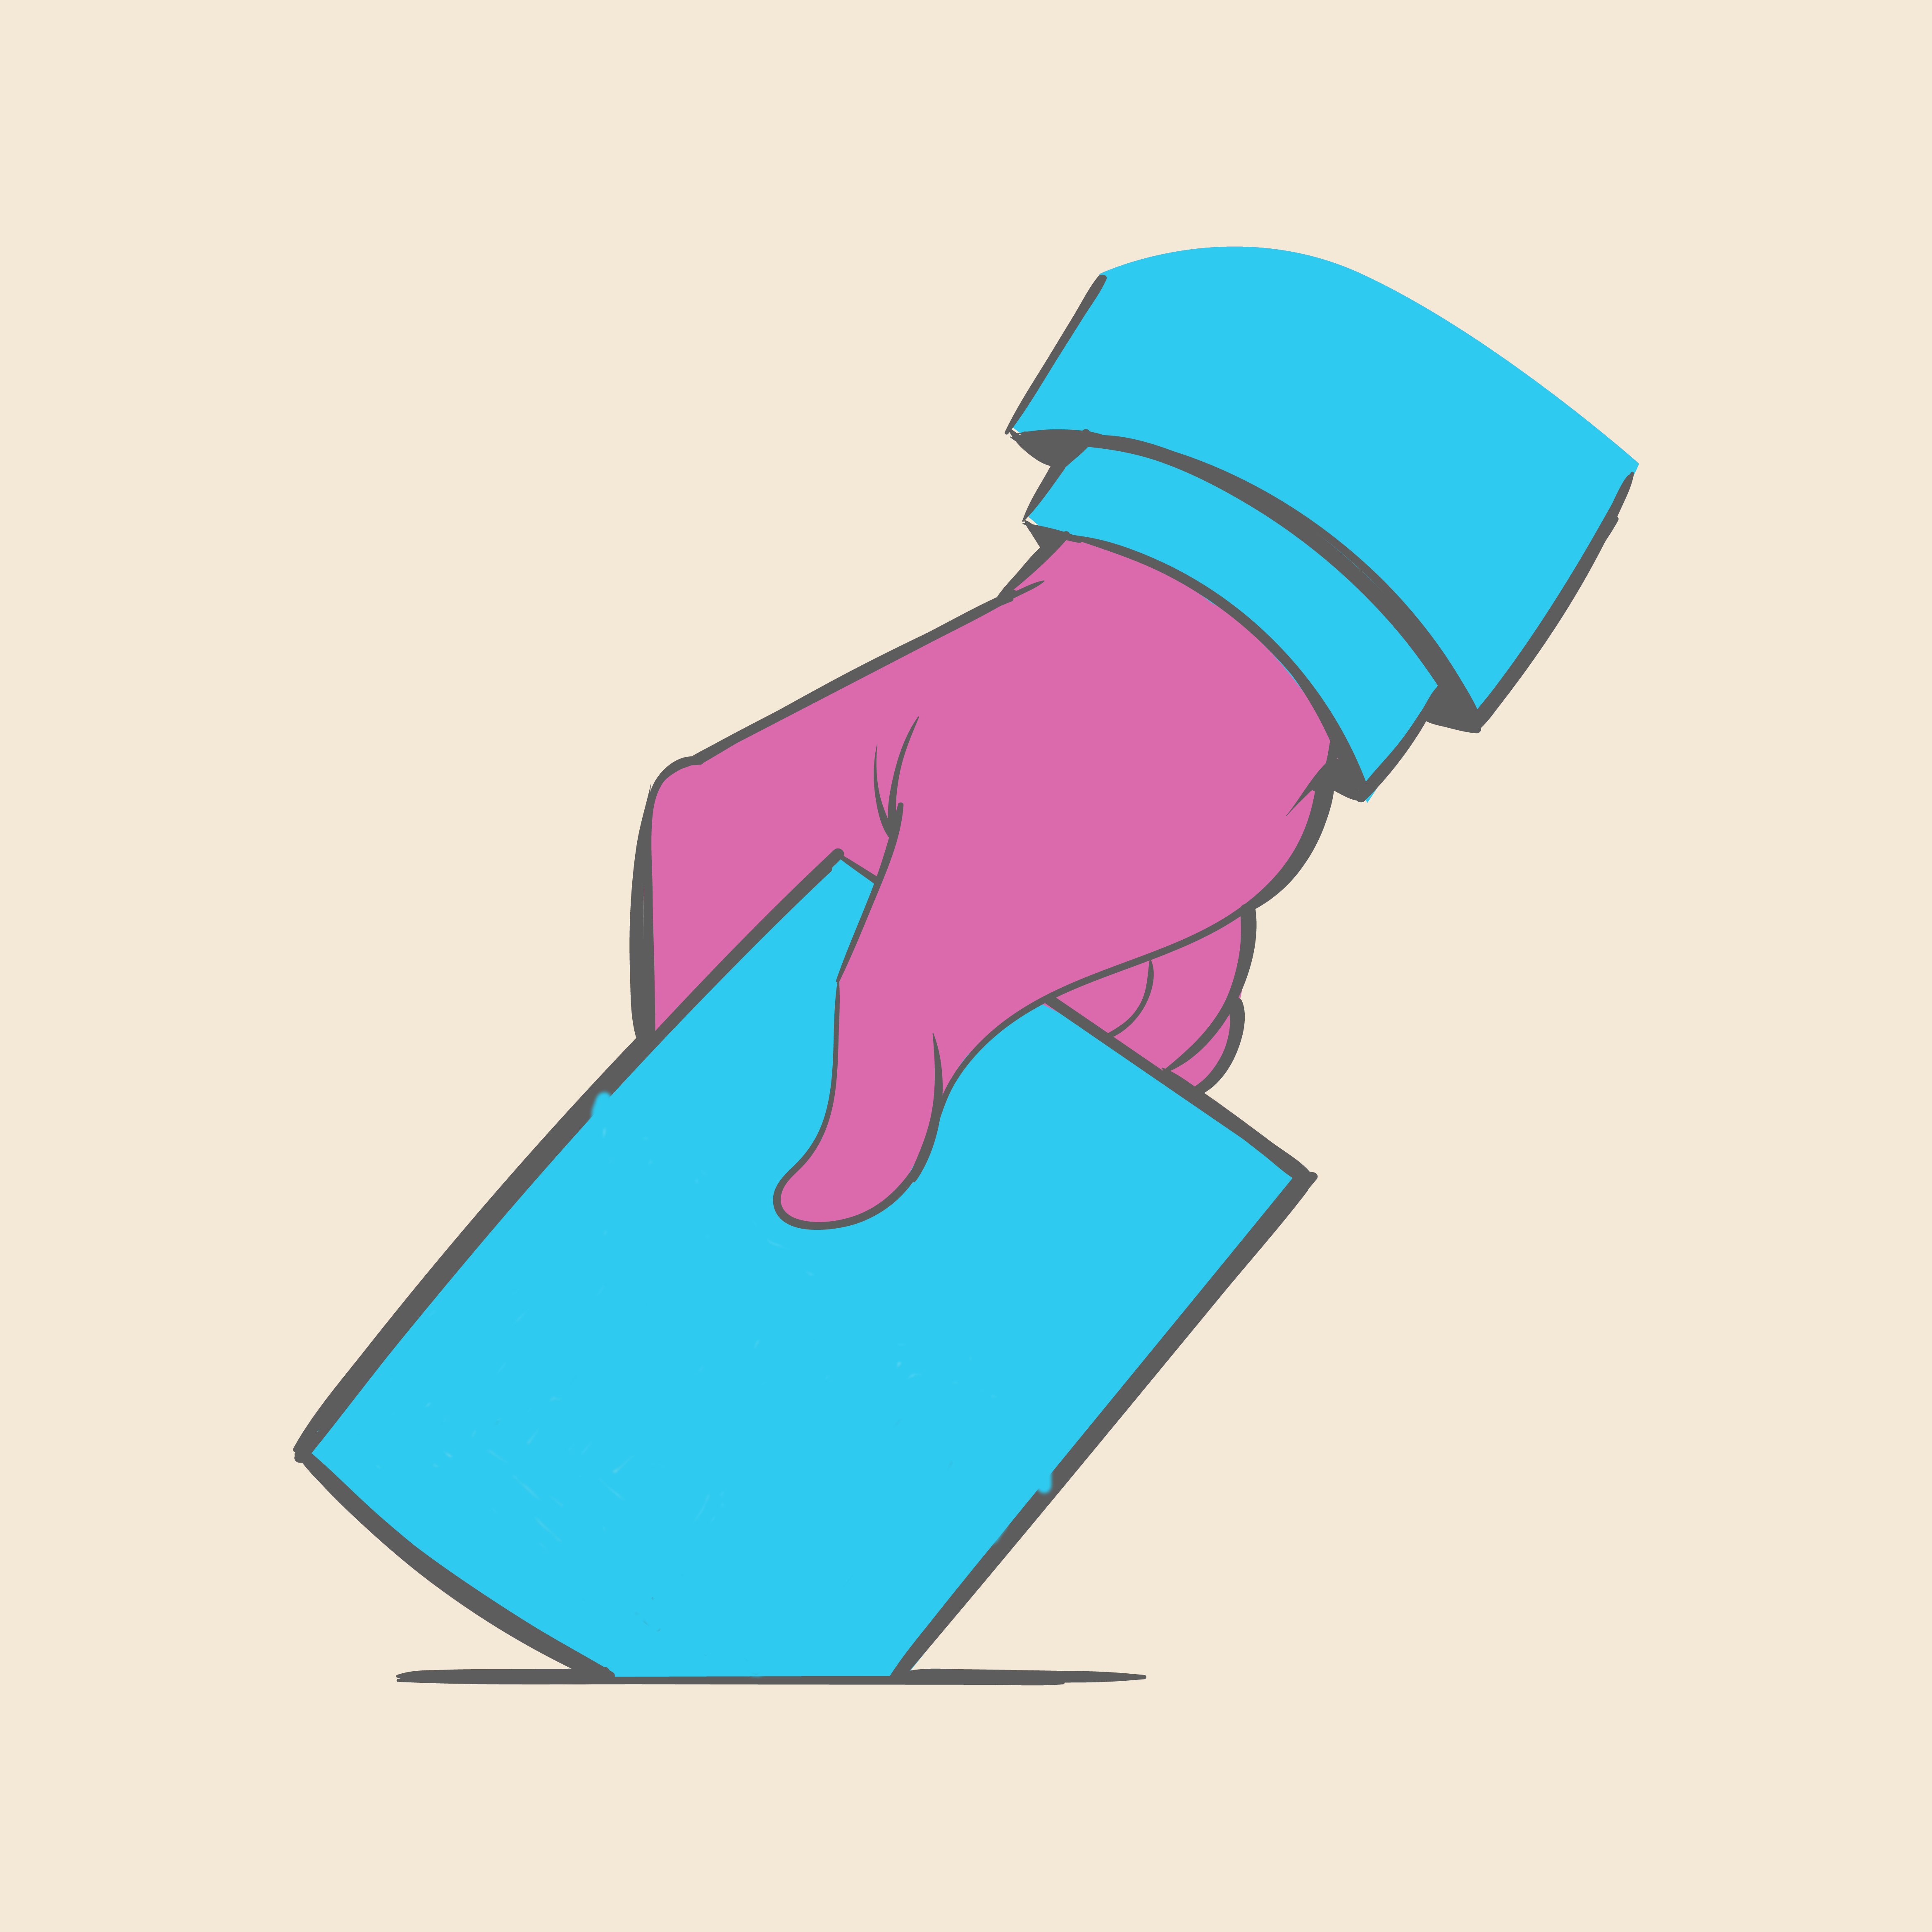
\includegraphics[width=.5\textwidth]{media/image84a.jpeg}
\end{center}

\begin{escolha}
\item
  Nenhuma.
\item
  A mesma que de sair um número ímpar.
\item
  Menor que a de sair um número ímpar.
\item
  Total.
\end{escolha}


\num{9} Um universítário recebeu seu boletim de notas. Veja a seguir.

\begin{figure}[htpb!]
\centering
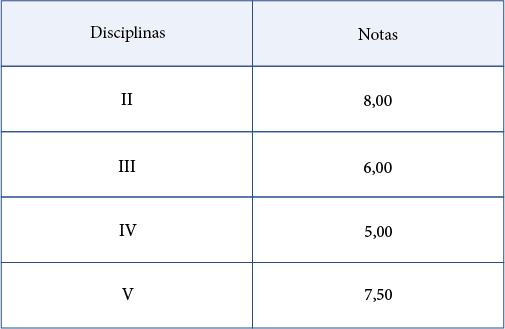
\includegraphics[width=.7\textwidth]{media/image85.png}
\end{figure}

\pagebreak
A nota mínima para aprovação em cada disciplina é 6,00. O estudante ficou exatamente na nota de aprovação na disciplina

%\begin{multicols}{2}
\begin{escolha}
\item
  I.
\item
  II.
\item
  III.
\item
  IV.
\end{escolha}
%\end{multicols}


\num{10} Em uma seletiva para a fase final da prova de 100 metros livres de
natação, oito atletas tiveram os tempos apresentados a seguir.

\begin{figure}[htpb!]
\centering
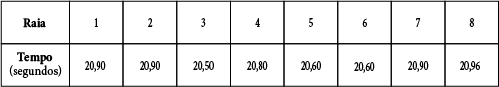
\includegraphics[width=\textwidth]{media/image86.png}
\end{figure}

Apenas os três mais velozes passam para a próxima fase. Os atletas classificados foram os das raias

%\begin{multicols}{2}
\begin{escolha}
\item
  3, 1 e 8.
\item
  3, 5 e 6.
\item
  1, 7 e 8.
\item
  5, 6 e 7.
\end{escolha}
%\end{multicols}


\num{11} Um prêmio de R\$ 900,00 será dividido entre três pessoas como descrito a seguir.

\conteudo{
\begin{itemize}
\item
  O \textbf{primeiro colocado} receberá $\frac{2}{3}$ do prêmio;
\item
  O \textbf{segundo colocado} receberá $\frac{1}{5}$ do prêmio;
\item
  O \textbf{terceiro colocado} receberá o restante do prêmio.
\end{itemize}
}

Sendo assim, pode-se afirmar que o segundo colocado receberá

\begin{multicols}{2}
\begin{escolha}
\item
  R\$ 300,00.
\item
  R\$ 200,00.
\item
  R\$ 180,00.
\item
  R\$ 50,00.
\end{escolha}
\end{multicols}

\pagebreak
\num{12} Durante um treino de futebol, Camilo acertou 18 pênaltis dos 36 que
bateu. Com isso, percebe-se que ele acertou em

\begin{center}
\includegraphics[width=.8\textwidth]{media/image86a_.jpeg}
\end{center}

%\begin{multicols}{2}
\begin{escolha}
\item
  $\frac{5}{10}$ das tentativas.
\item
  $\frac{1}{4}$ das tentativas.
\item
  $\frac{2}{3}$ das tentativas.
\item
  $\frac{1}{10}$ das tentativas.
\end{escolha}
%\end{multicols}


\num{13} Uma poltrona reclinável moderna possui o assento com quatro opções de posição
diferentes, e o encosto pode ser usado em seis opções de posição diferentes. Combinando-se uma posição do assento com uma posição do encosto, quantas combinações existem?

%\begin{multicols}{2}
\begin{escolha}
\item
  10.
\item
  16.
\item
  24.
\item
  36.
\end{escolha}
%\end{multicols}

\pagebreak

\num{14} Lucas, com o auxílio de seu professor, está montando no laboratório de
robótica um supersistema de transmissão de dados. Para isso, ele
precisa de 7 metros de fio de cobre, cortados em pedaços menores de 0,14
metro de comprimento. Ela já possui 24 pedaços no tamanho desejado. Quantos pedaços ainda
faltam para ele continuar a montar seu sistema?

\begin{center}
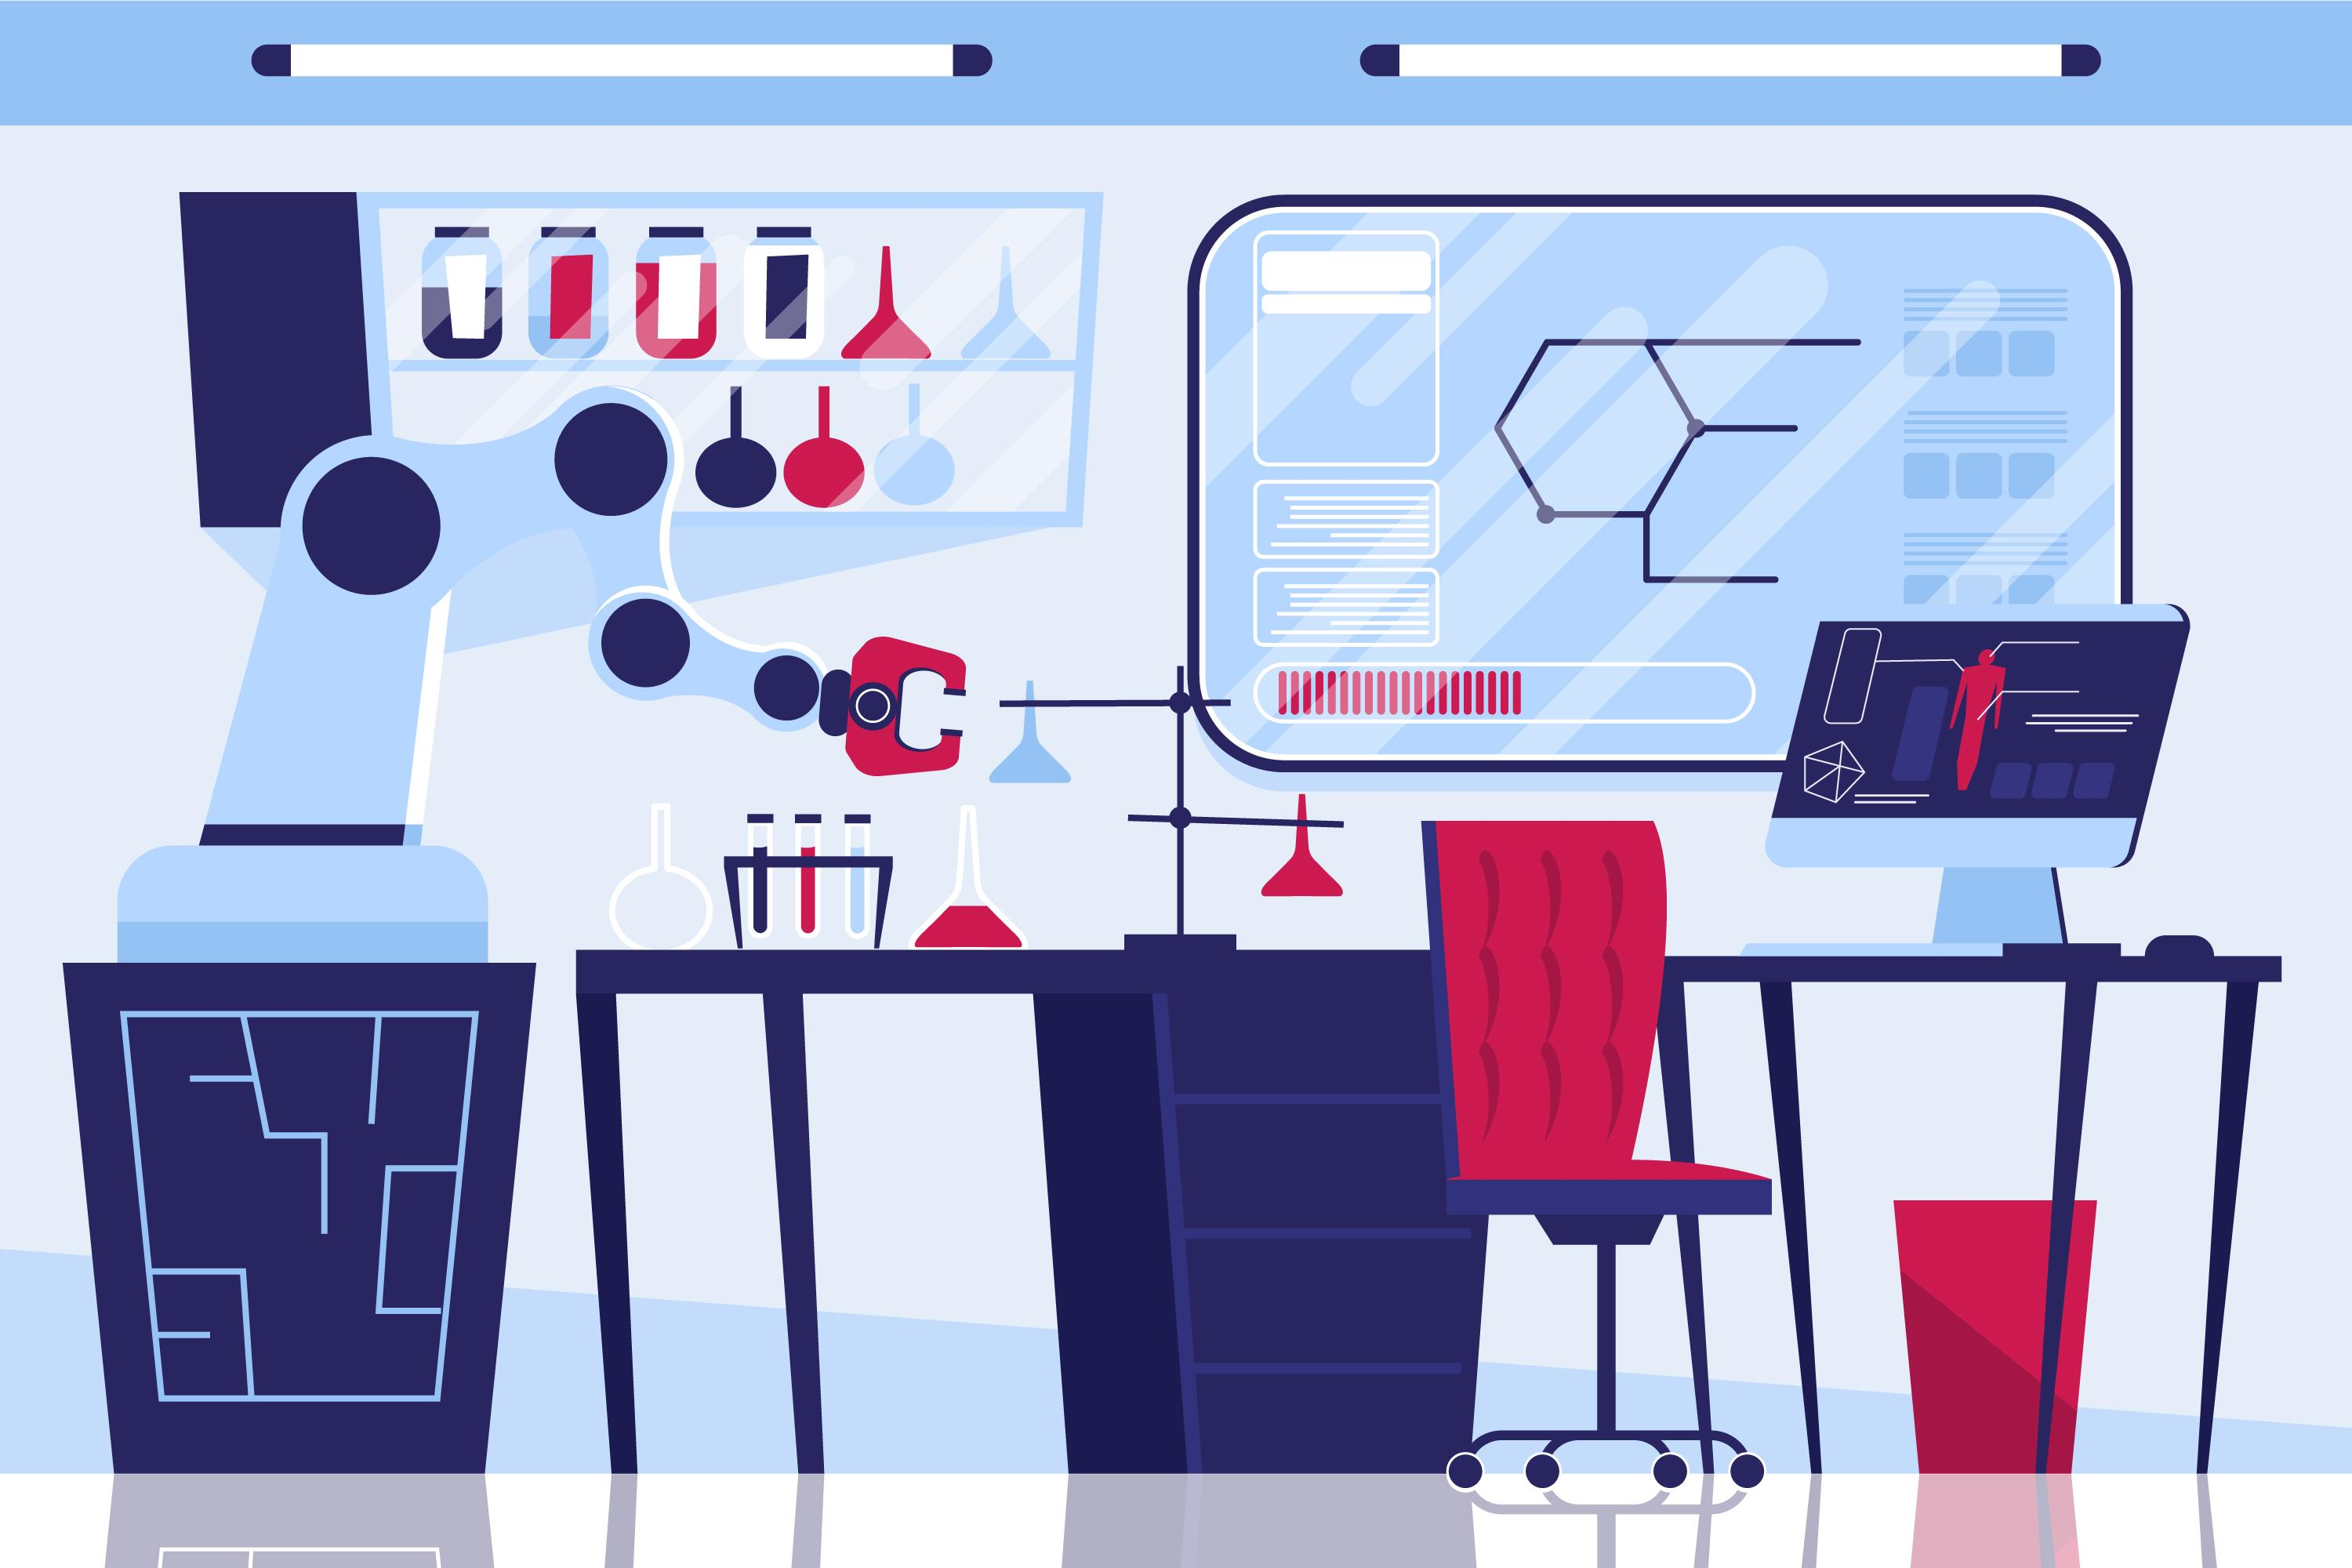
\includegraphics[width=.8\textwidth]{media/image86b_.jpeg}
\end{center}

%\begin{multicols}{2}
\begin{escolha}
\item
  8.
\item
  26.
\item
  42.
\item
  50.
\end{escolha}
%\end{multicols}


\num{15} O relógio de rua de determinada cidade está marcando a temperatura
de 32 graus Celsius. Esse valor, multiplicado por dez mil, é escrito de que forma?

%\begin{multicols}{2}
\begin{escolha}
\item Trezentos e vinte.
\item Três mil e duzentos.
\item Trinta e dois mil.
\item Trezentos e vinte mil.
\end{escolha}
%\end{multicols}
\pagebreak

\vspace*{-3.4cm}
\hspace*{-3.7cm}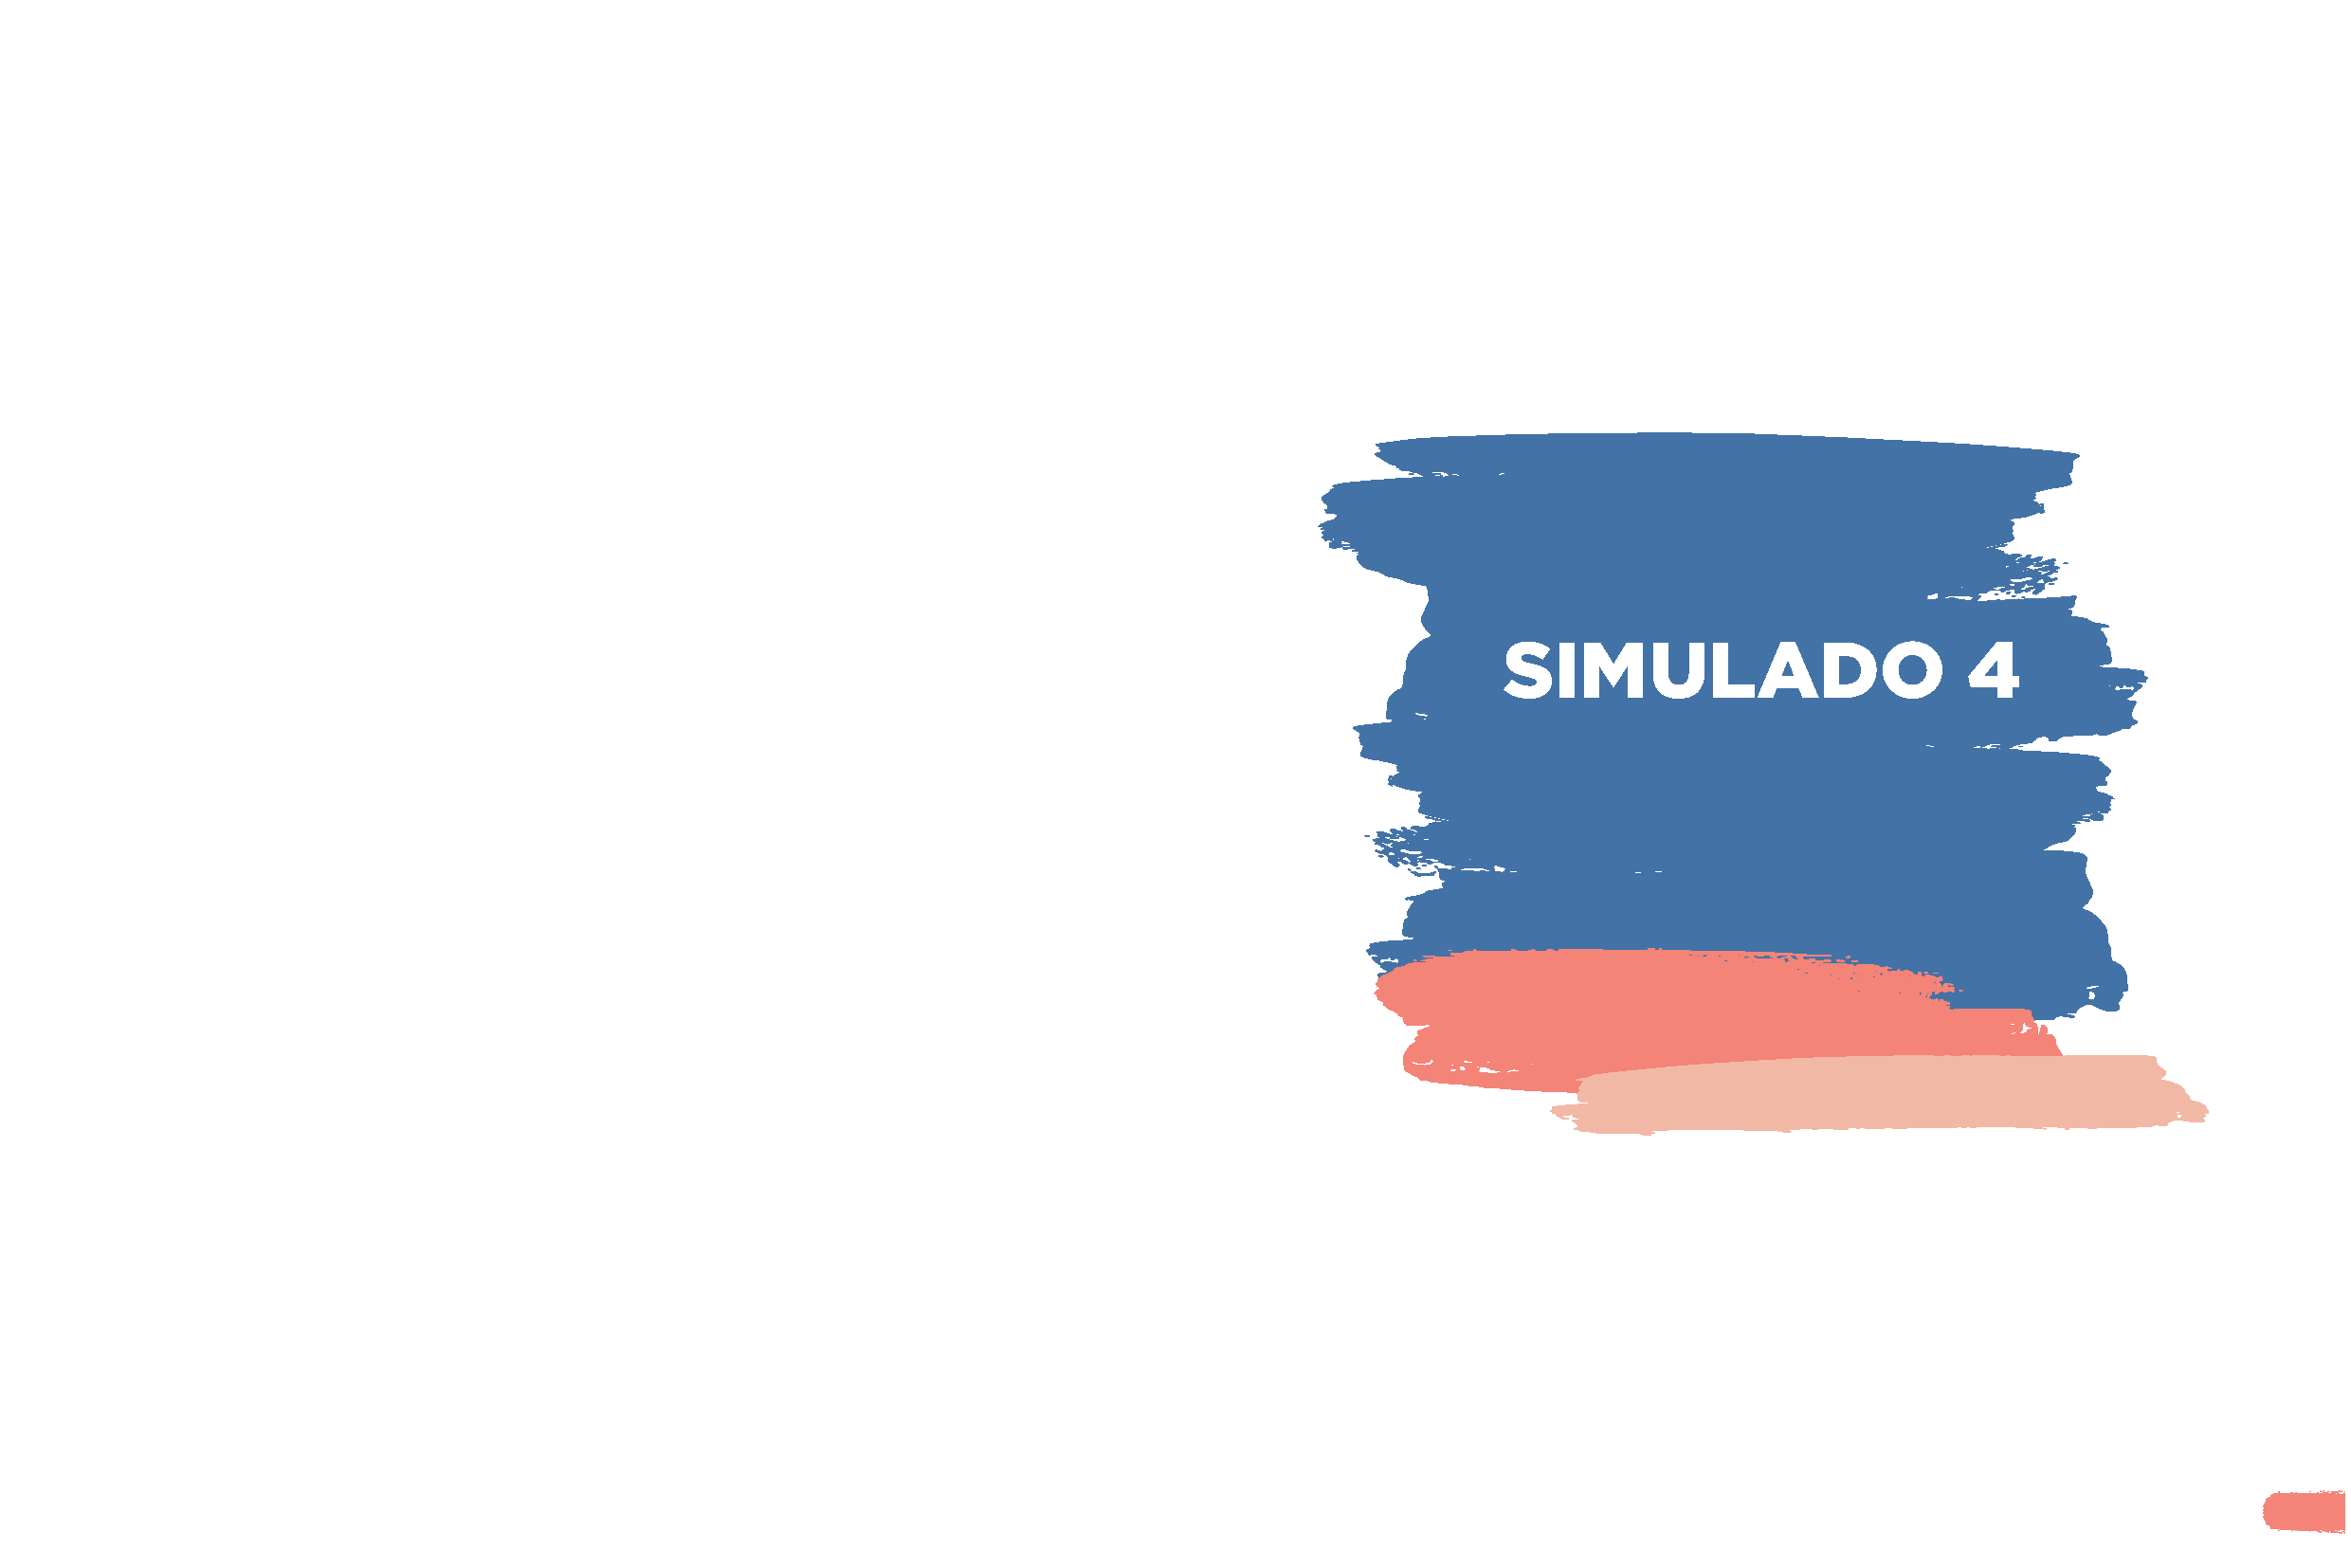
\includegraphics[scale=1]{../watermarks/4simulado5ano.pdf}
\addcontentsline{toc}{chapter}{Simulado 4}
\markboth{Simulado 4}{}

\pagebreak
\num{1} Ana Luísa viu uma placa afixada na porta de uma obra de construção civil. A placa trazia o texto reproduzido a seguir.

\begin{center}

\includegraphics[width=\textwidth]{media/image86a.jpeg}
\end{center}

\conteudo{
\textbf{Um novo empreendimento}

\textit{Condomínio Casa do Verde}, sua nova casa no Bairro das Graças.

Faltam 1.249 dias para entregarmos o prédio pronto para você morar!
}

O número que aparece nessa placa pode ser decomposto de que forma?

\begin{escolha}
\item (500 x 2) + 100 + 100 + 40 + 9
\item 1.000 + 100 + 49  
\item 500 + 500 + 100 + 40 + 10  
\item 500 + 500 + (50 x 4) + 40  
\end{escolha}

\pagebreak
\num{2} Jorge foi passar as férias no sítio pertencente à sua família. Chegando lá,
correu até a horta e colheu 
10 dezenas de pés de rúcula, 
2 centenas de espiga de milho, 
8 dezenas de tomate,
7 unidades de cebola e 
3 pepinos.
O total de itens colhidos é

\begin{center}
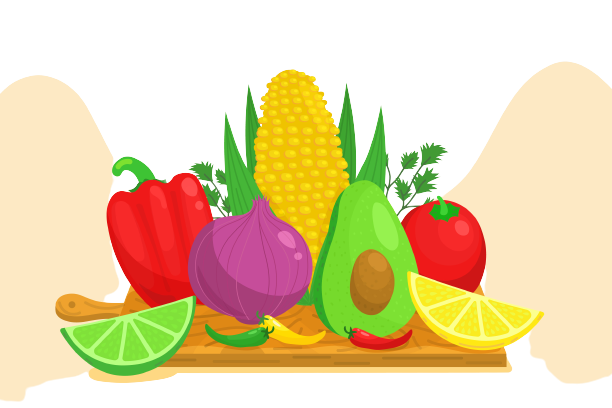
\includegraphics[width=\textwidth]{media/image86b.png}
\end{center}

\begin{escolha}
\item
  201.
\item
  258.
\item
  390.
\item
  673.
\end{escolha}


\num{3} Geraldo queria enviar um presente ao amigo José, que se mudou de cidade. Ele
sabia a cidade para qual o amigo havia se mudado, além do nome na rua, mas
não sabia o número da casa. Geraldo então enviou uma mensagem ao
amigo perguntando o número da casa. José respondeu da maneira mostrada a seguir.

\conteudo{
Como é nosso costume antigo, aí vai um enigma:\\
\textbf{O número da casa é: 4 + 2 x (16 -- 9) + 8 : 2.}
}

\pagebreak
Qual é o número da casa de José?

%\begin{multicols}{2}
\begin{escolha}
\item
  14.
\item
  20.
\item
  22.
\item
  28.
\end{escolha}
%\end{multicols}

\num{4} Arnaldo esqueceu um dos números que faz parte da senha do cofre que
possui em sua casa. Ele lembra que a senha era composta de 6 números e
que os números da senha formam a seguinte sequência (2, 102, 202,
A, 402, 502), em que A é o número que ele esqueceu. O número A é


\begin{center}

\includegraphics[width=.7\textwidth]{media/image86c.jpeg}
\end{center}

\begin{escolha}
\item
  o dobro de 150.
\item
  o antecessor de 303.
\item
  o sucessor de 251.
\item
  a metade de 500.
\end{escolha}

\pagebreak
\num{5} Observe os objetos a seguir.

\begin{figure}[htpb!]
\centering
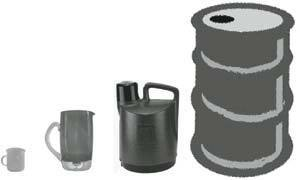
\includegraphics[width=.7\textwidth]{media/image87.jpg}
\end{figure}

Em qual desses objetos caberiam pelo menos 40 litros de água?

%\begin{multicols}{2}
\begin{escolha}
\item
  Na caneca.
\item
  Na jarra.
\item
  No garrafão.
\item
  No tambor.
\end{escolha}
%\end{multicols}


\num{6} Um clube de futebol está criando uma nova bandeira, e decidiram que ela seria composta de duas cores diferentes, tendo sido sugeridas seis cores
diferentes para serem utilizadas. Qual é a quantidade total de combinações
diferentes de cores para compor essa bandeira?

\begin{escolha}
\item
  8.
\item
  15.
\item
  30.
\item
  36.
\end{escolha}


\num{7} Rafael foi a uma papelaria e comprou um livro por R\$ 35,00 e uma caneta
por R\$ 3,00. Das alternativas a seguir, qual pode representar as cédulas
e moedas que Rafael utilizou para pagar, sem troco?

\begin{escolha}
\item
  1 cédula de 10 reais, 5 cédulas de 5 reais e 3 moedas de 1 real.
\item
  1 cédula de 10 reais, 4 cédulas de 5 reais e 3 moedas de 1 real.
\item
  2 cédulas de 10 reais, 1 cédula de 5 reais e 3 moedas de 1 real.
\item
  2 cédulas de 10 reais, 2 cédulas de 5 reais e 2 moedas de 1 real.
\end{escolha}


\num{8} Alana resolveu trocar todas as moedas que estavam em seu cofrinho por uma
única cédula. Ela tinha no cofrinho 10 moedas de 5 centavos, 5 moedas de
50 centavos, 70 moedas de 10 centavos e 10 moedas de 1 real. Ela vai trocar por uma cédula de

\begin{escolha}
\item R\$ 2,00.
\item R\$ 5,00.
\item R\$ 10,00.
\item R\$ 20,00.
\end{escolha}


\num{9} Um agricultou tem quatro mudas de uma planta que pode dar flores em três cores diferentes: amarela, rosa ou laranja. No viveiro, ele tem a mesma quantidade de mudas de cada cor de flor. Assim, na primeira vez, retirando uma muda ao acaso, ele tem

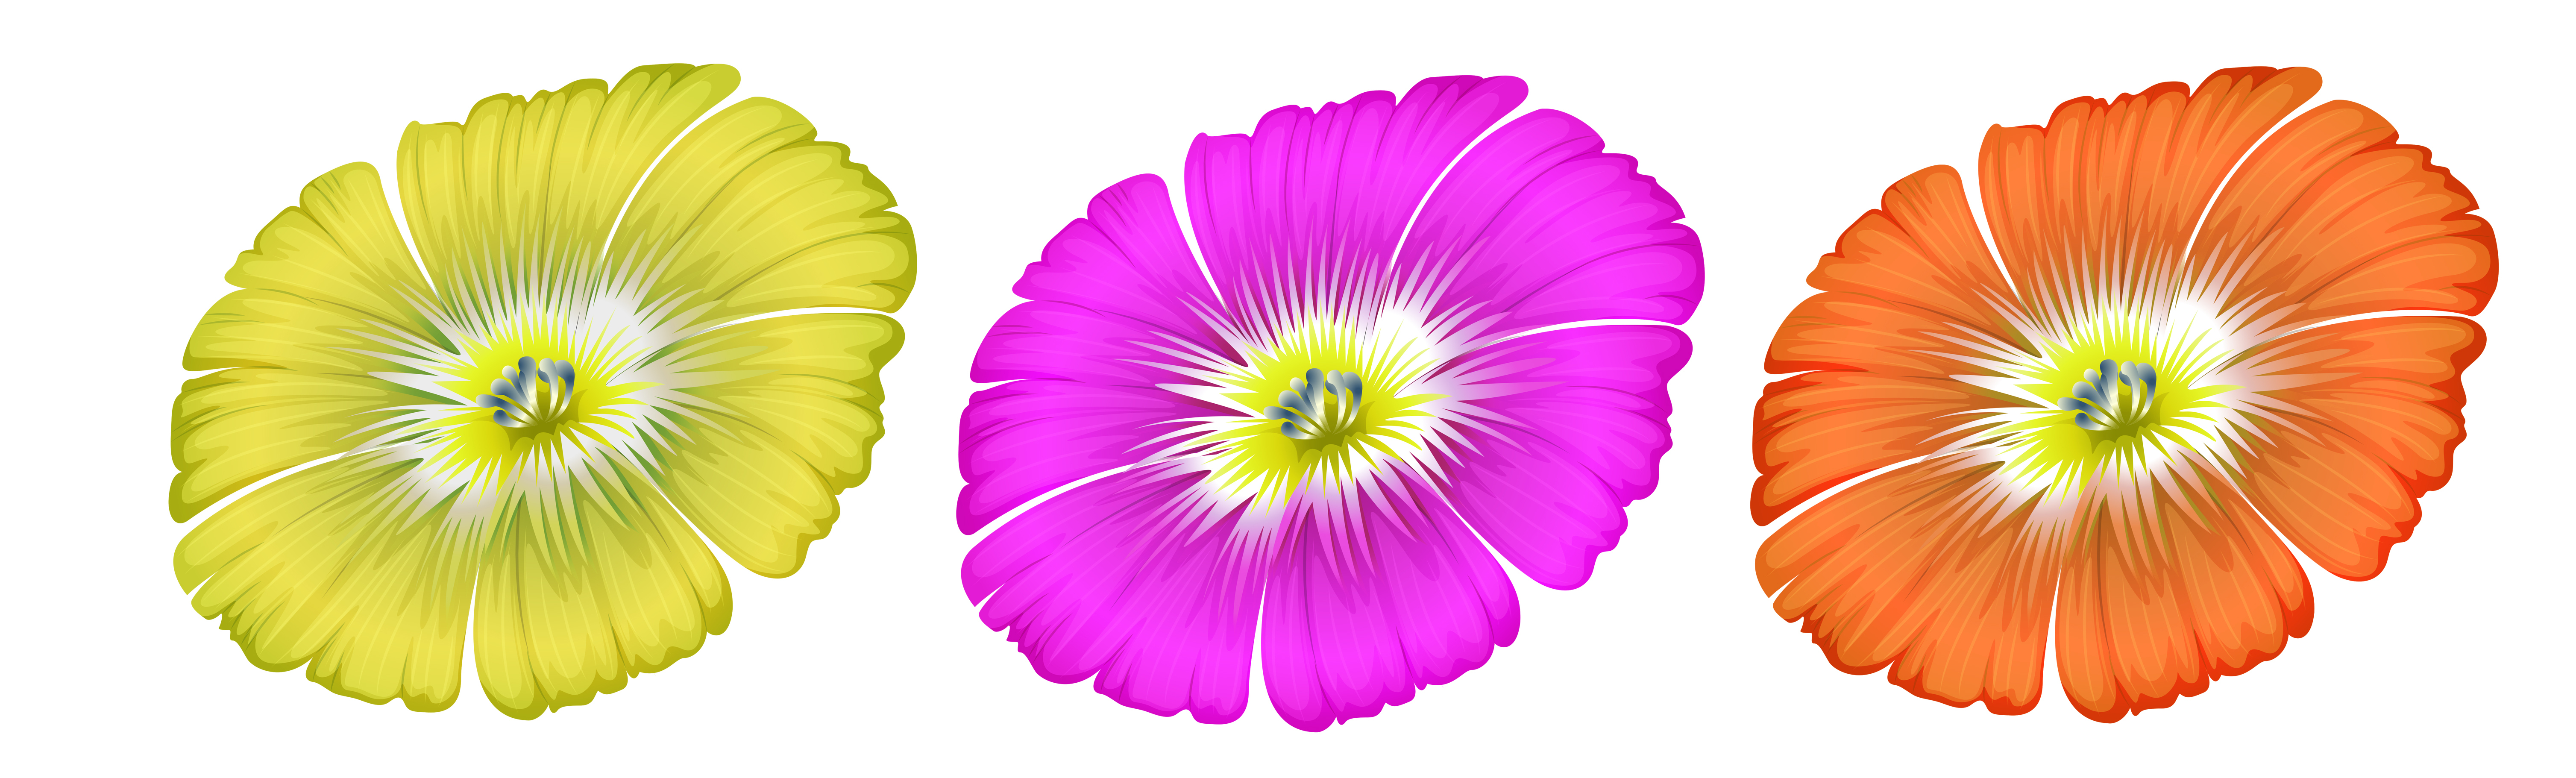
\includegraphics[width=\textwidth]{media/image87a.jpeg}

\begin{escolha}
\item mais chance de pegar uma muda com flor rosa.
\item mais chance de pegar uma muda com flor amarela.
\item mais chance de pegar uma muda com flor laranja.
\item as mesmas chances de pegar uma muda com uma das cores.
\end{escolha}


\num{10} Em uma competição de saltos ornamentais, cada atleta tem direito a três saltos,
e sua pontuação final é dada pela soma dos pontos obtidos após cada salto. Ganha a prova quem
fizer o maior número de pontos no total. A tabela a seguir mostra as notas obtidas por 5 atletas, A, B, C, D e E, nos seus respectivos saltos.

\pagebreak
\begin{figure}[htpb!]
\centering
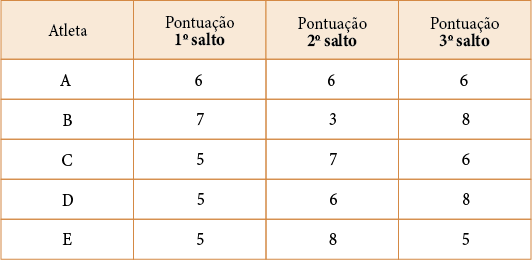
\includegraphics[width=\textwidth]{media/image88.png}
\end{figure}

Os atletas que empataram foram

\begin{multicols}{2}
\begin{escolha}
\item
  A e B e E
\item
  A, B e C.
\item
  C e D e E
\item
  A, B, C e E.
\end{escolha}
\end{multicols}

\num{11} Em uma prova de automobilismo, o competidor que estava em primeiro lugar
sofreu com falta de combustível e precisou abandonar a prova quando já
tinha completado $\frac{4}{7}$ da prova de 77 voltas no total. Pode-se dizer que,
no momento em que ele abandonou a prova, ainda faltavam para a corrida
terminar

\vspace{2em}
\begin{center}
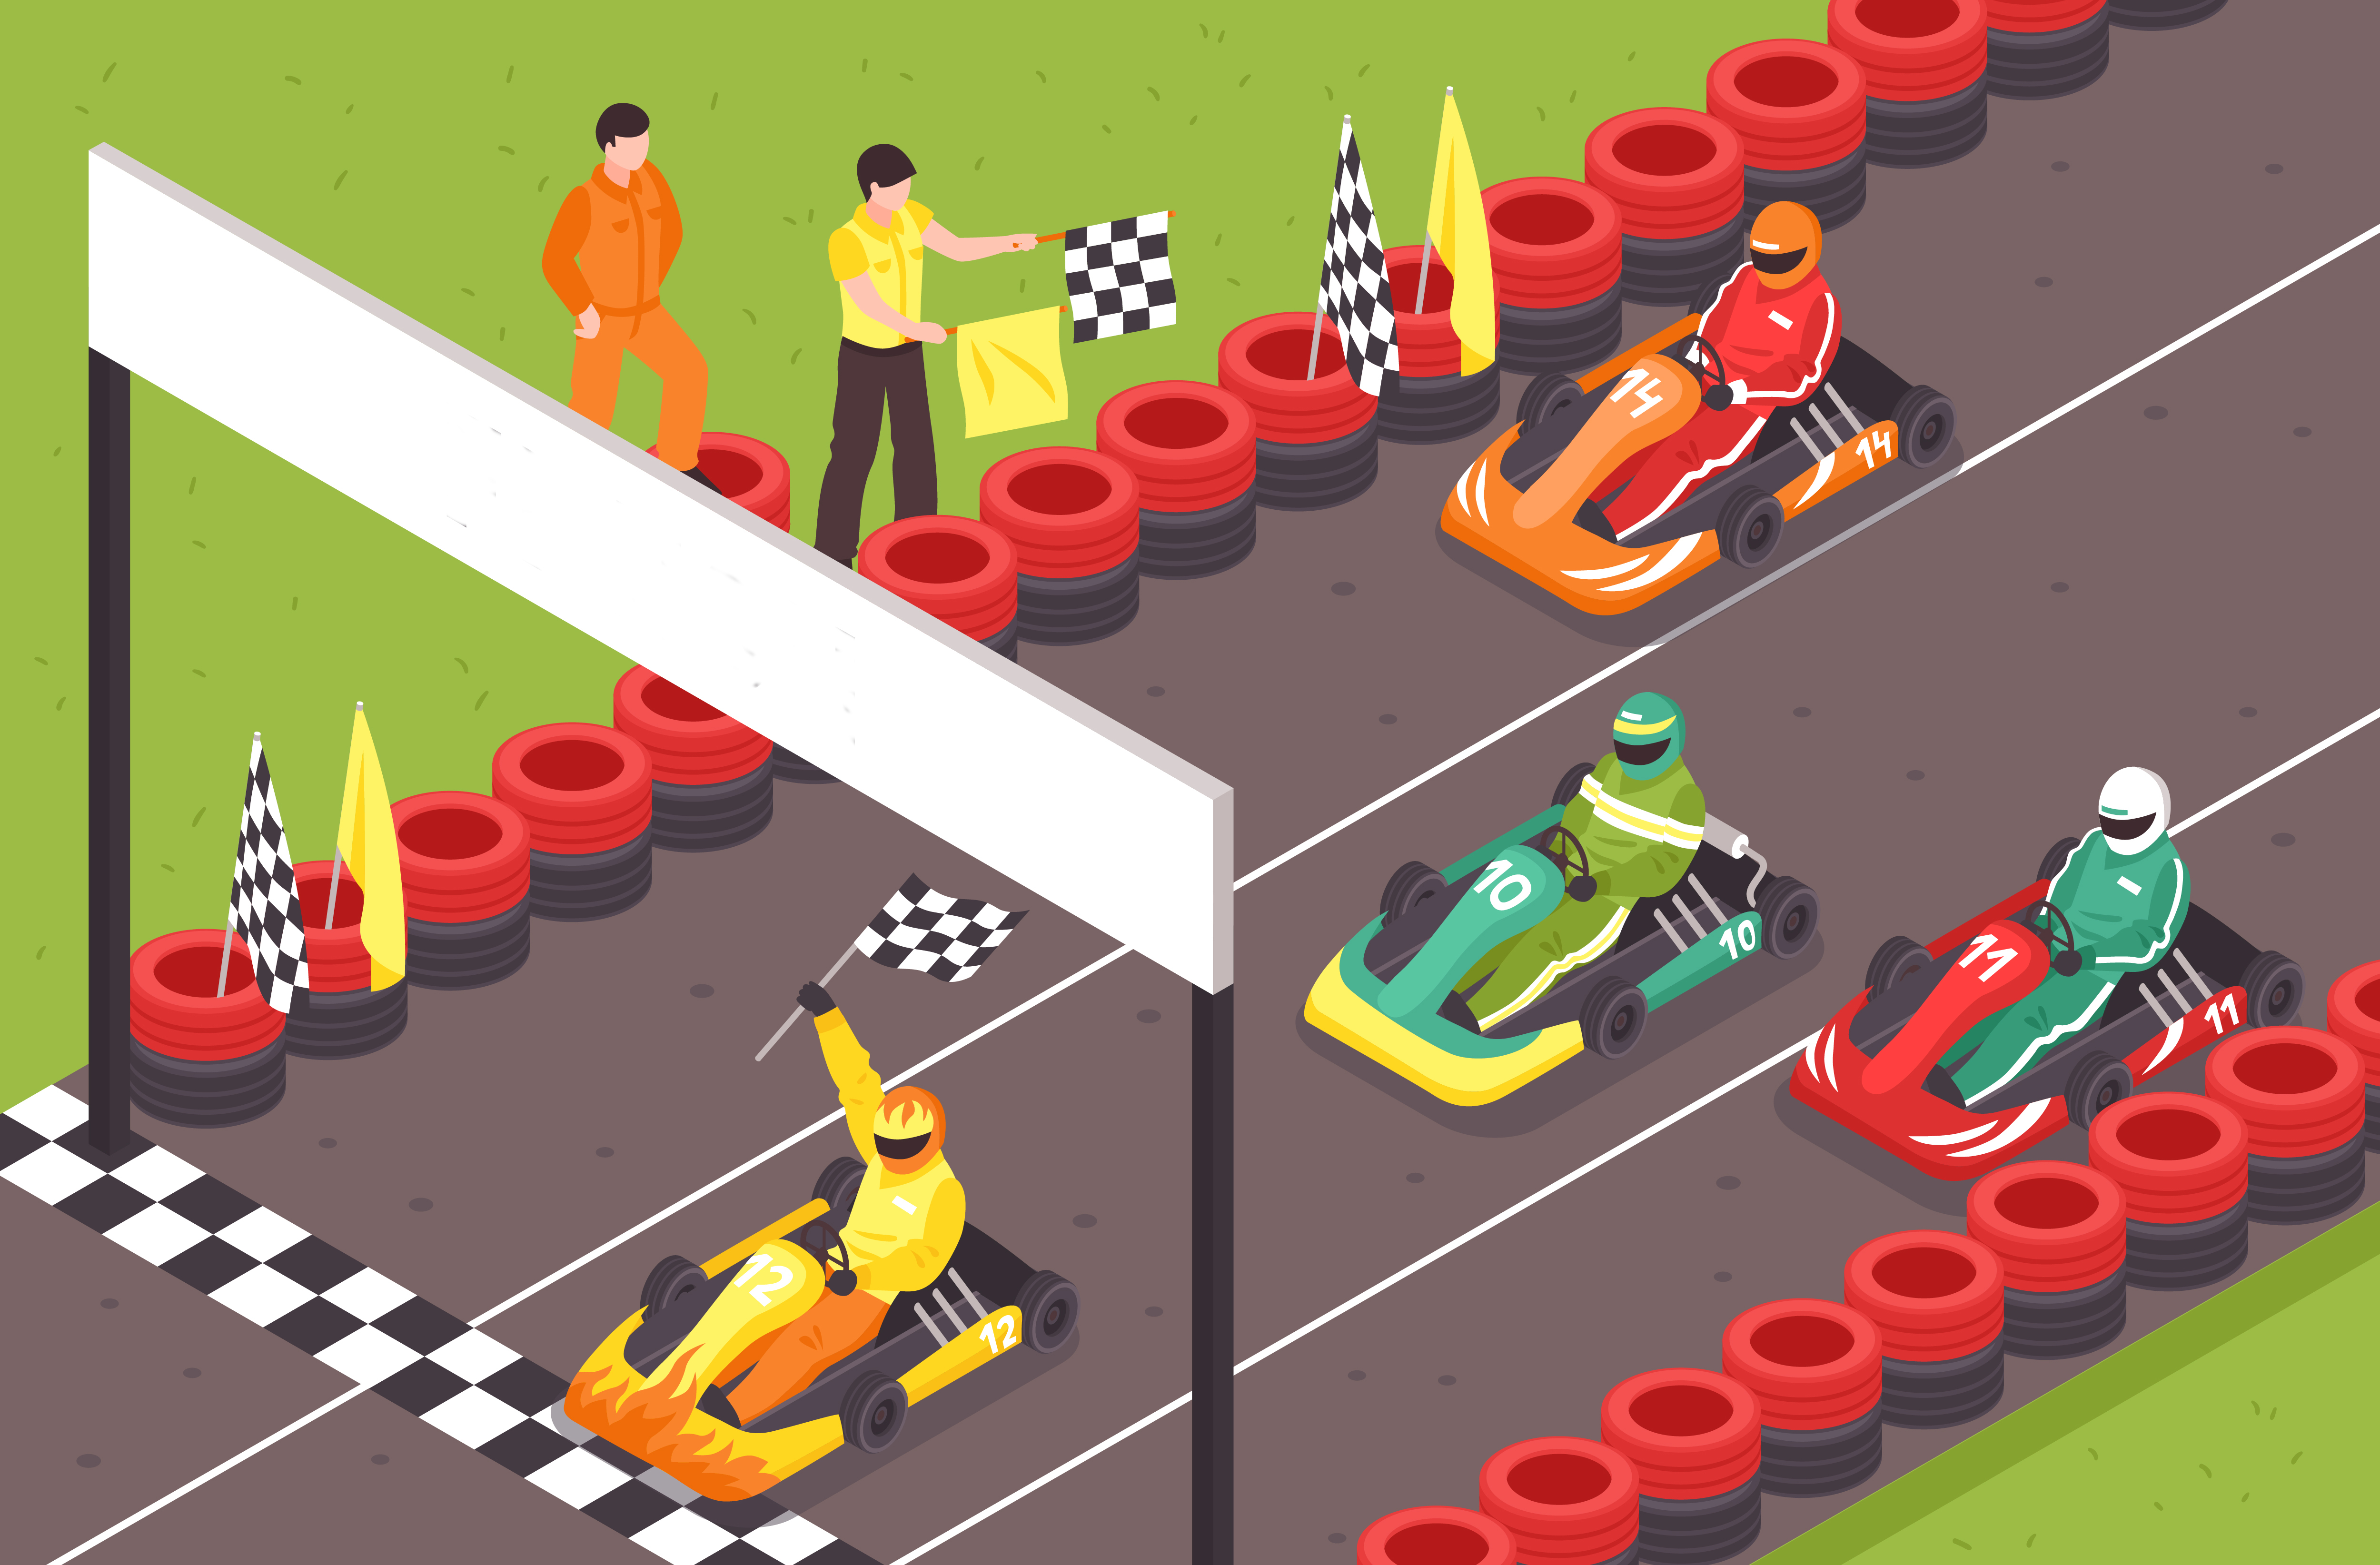
\includegraphics[width=.7\textwidth]{media/image88a.jpeg}
\end{center}

\pagebreak
\begin{escolha}
\item
  11 voltas.
\item
  22 voltas.
\item
  33 voltas.
\item
  44 voltas.
\end{escolha}


\num{12} Em um mapa, a distância de 2.000 km entre duas cidades foi representada
por um segmento, em centímetros, equivalente a $\frac{1}{250}$ do número que
representa a distância em quilômetros. Sendo assim, podemos dizer que, no
mapa, o segmento terá

\vspace{2em}
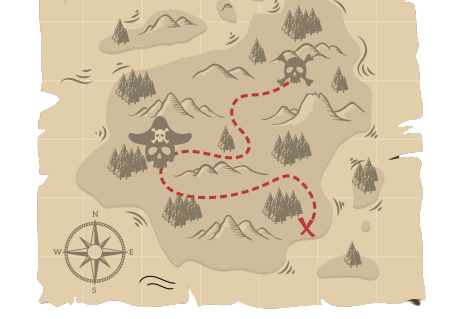
\includegraphics[width=.8\textwidth]{media/image88b.png}

\begin{escolha}
\item
  8 centímetros.
\item
  16 centímetros.
\item
  50 centímetros.
\item
  250 centímetros.
\end{escolha}


\num{13} Quantos números de três algarismos podemos compor com os 1, 2, 3, 4, 5, 6, 7, 8 e 9 de forma que nenhum algarismo se repita?

\begin{multicols}{2}
\begin{escolha}
\item
  243.
\item
  358.
\item
  504.
\item
  729.
\end{escolha}
\end{multicols}

\pagebreak
\num{14} Alexandre foi até uma loja comprar um tênis e foi informado de que o valor
era de R\$ 322,00. Após algum tempo de negociação, o gerente da loja decidiu
abaixar o preço em R\$ 42,00 e ainda permitir o parcelamento do restante em 4 parcelas iguais.
Qual é o valor de cada parcela?

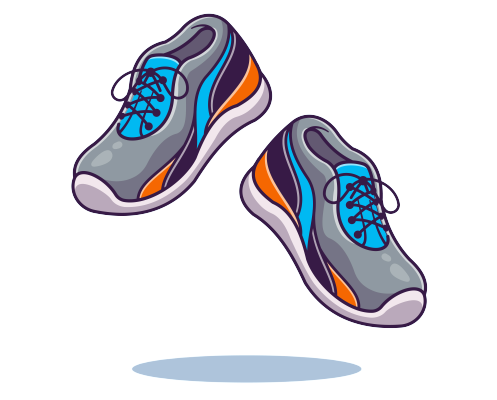
\includegraphics[width=.8\textwidth]{media/image88c.png}

\begin{escolha}
\item
  R\$ 280,00.
\item
  R\$ 120,00.
\item
  R\$ 70,00.
\item
  R\$ 30,00.
\end{escolha}


\num{15} O relógio digital de Ana está marcando 12h03.
O número, em algarismos romanos, que representa só o número das horas é

\begin{escolha}
\item
  IIX.
\item
  IXX.
\item
  XII.
\item
  XXI.
\end{escolha}


